\chapter{Simulation}

\begin{figure}[H]
\centering
\includegraphics[width=\textwidth, page=1]{Simulation}
\label{fig:OverallSimulation}
\caption{Overall view of the system being simulated}
\end{figure}


\begin{figure}[H]
\centering
\begin{subfigure}[t]{0.49\textwidth}
    \centering
\includegraphics[width=\textwidth, page=2]{Simulation}
    \caption{Downsampling system}
    \label{fig:DownsamplingSimulation}
\end{subfigure}
\begin{subfigure}[t]{0.49\textwidth}
    \centering
\includegraphics[width=\textwidth, page=11]{Simulation}
    \caption{Upsampling system}
    \label{fig:UpsamplingSimulation}
\end{subfigure}
\begin{subfigure}[t]{\textwidth}
    \centering
\includegraphics[width=\textwidth, page=13]{Simulation}
    \caption{RMS Compressor}
    \label{fig:RMSCompressorSimulation}
\end{subfigure}
\label{fig:SubsystemSimulation}
\caption{View of the subsystems found in figure \ref{fig:OverallSimulation}}
\end{figure}


\section{10 second simulation}
\begin{figure}[H]
\centering
\begin{subfigure}[t]{0.49\textwidth}
    \centering
    \tikzsetnextfilename{Band1Simulation}
    % This file was created by matlab2tikz.
%
%The latest updates can be retrieved from
%  http://www.mathworks.com/matlabcentral/fileexchange/22022-matlab2tikz-matlab2tikz
%where you can also make suggestions and rate matlab2tikz.
%
\definecolor{mycolor1}{rgb}{0.00000,0.44700,0.74100}%
\definecolor{mycolor2}{rgb}{0.85000,0.32500,0.09800}%
\definecolor{mycolor3}{rgb}{0.00,0.00,0.00}%
%\definecolor{mycolor3}{rgb}{0.92900,0.69400,0.12500}%
%
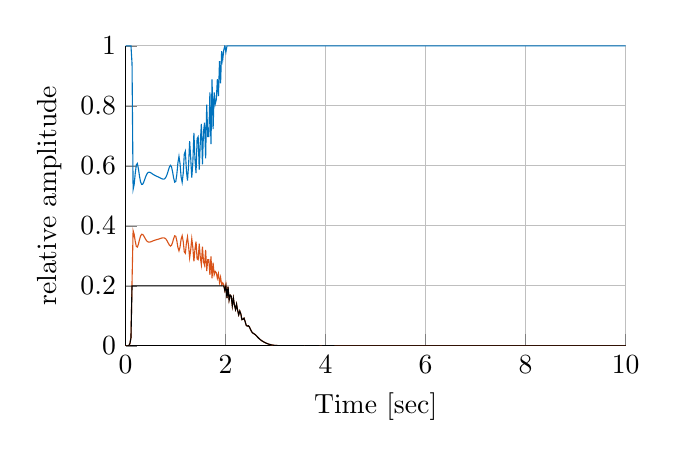
\begin{tikzpicture}

\begin{axis}[%
width=2.5in,
height=1.5in,
scale only axis,
xmin=0,
xmax=10,
xlabel={Time [sec]},
xmajorgrids,
ymin=0,
ymax=1,
ylabel={relative amplitude},
ymajorgrids,
axis background/.style={fill=white},
axis x line*=bottom,
axis y line*=left
]
\addplot [color=mycolor1,solid,forget plot]
  table[row sep=crcr]{%
0	1\\
0.0213333333333333	1\\
0.0426666666666667	1\\
0.064	1\\
0.0853333333333333	1\\
0.106666666666667	1\\
0.128	0.94052925665693\\
0.149333333333333	0.521312680503569\\
0.170666666666667	0.5379588233159\\
0.192	0.57419394721995\\
0.213333333333333	0.603097527850566\\
0.234666666666667	0.607805804615097\\
0.256	0.589681384652847\\
0.277333333333333	0.565090076692022\\
0.298666666666667	0.546503259345334\\
0.32	0.537967178813041\\
0.341333333333333	0.538647529342774\\
0.362666666666667	0.545723419380477\\
0.384	0.555784315505287\\
0.405333333333333	0.565683829355308\\
0.426666666666667	0.573226306250534\\
0.448	0.577515793803996\\
0.469333333333333	0.578793065375333\\
0.490666666666667	0.577922744291202\\
0.512	0.57587483190482\\
0.533333333333333	0.573415460073872\\
0.554666666666667	0.571013871586326\\
0.576	0.568875895885298\\
0.597333333333333	0.56702106224806\\
0.618666666666667	0.565359523899438\\
0.64	0.563756104458674\\
0.661333333333333	0.562084790241028\\
0.682666666666667	0.560281826931268\\
0.704	0.558403091421754\\
0.725333333333333	0.556683604111594\\
0.746666666666667	0.55558569430147\\
0.768	0.555809917933225\\
0.789333333333333	0.558230318202923\\
0.810666666666667	0.563698044576393\\
0.832	0.57262747173052\\
0.853333333333333	0.584266636511101\\
0.874666666666667	0.595740850284354\\
0.896	0.601739195746008\\
0.917333333333333	0.596784327862422\\
0.938666666666667	0.580338630240974\\
0.96	0.559534666479262\\
0.981333333333333	0.545479971587961\\
1.00266666666667	0.547874575750174\\
1.024	0.571563894043458\\
1.04533333333333	0.609635460125638\\
1.06666666666667	0.631588867885951\\
1.088	0.607280896148104\\
1.10933333333333	0.562948465029064\\
1.13066666666667	0.545117792814257\\
1.152	0.575461551636541\\
1.17333333333333	0.639318227989924\\
1.19466666666667	0.648717930981153\\
1.216	0.582538952922978\\
1.23733333333333	0.550895424081265\\
1.25866666666667	0.601738671277135\\
1.28	0.681897426710945\\
1.30133333333333	0.626736186486799\\
1.32266666666667	0.560394081487352\\
1.344	0.610663732511975\\
1.36533333333333	0.710004434804772\\
1.38666666666667	0.621454379983968\\
1.408	0.575609876707623\\
1.42933333333333	0.690605509888366\\
1.45066666666667	0.696849224691197\\
1.472	0.587113439575133\\
1.49333333333333	0.678936183125104\\
1.51466666666667	0.739839405019572\\
1.536	0.605093340716769\\
1.55733333333333	0.713990862546606\\
1.57866666666667	0.744113209775967\\
1.6	0.625124457195537\\
1.62133333333333	0.803846862950313\\
1.64266666666667	0.69757168039577\\
1.664	0.697545544944081\\
1.68533333333333	0.845003389712843\\
1.70666666666667	0.671912302276424\\
1.728	0.887691672045862\\
1.74933333333333	0.722203076464605\\
1.77066666666667	0.84462248065369\\
1.792	0.806558911241585\\
1.81333333333333	0.820488607168327\\
1.83466666666667	0.888730521563202\\
1.856	0.832105402758059\\
1.87733333333333	0.949282503442451\\
1.89866666666667	0.874757860311495\\
1.92	0.982104604406591\\
1.94133333333333	0.953300933505307\\
1.96266666666667	0.98604684272416\\
1.984	1\\
2.00533333333333	0.978921617019547\\
2.02666666666667	1\\
2.048	1\\
2.06933333333333	1\\
2.09066666666667	1\\
2.112	1\\
2.13333333333333	1\\
2.15466666666667	1\\
2.176	1\\
2.19733333333333	1\\
2.21866666666667	1\\
2.24	1\\
2.26133333333333	1\\
2.28266666666667	1\\
2.304	1\\
2.32533333333333	1\\
2.34666666666667	1\\
2.368	1\\
2.38933333333333	1\\
2.41066666666667	1\\
2.432	1\\
2.45333333333333	1\\
2.47466666666667	1\\
2.496	1\\
2.51733333333333	1\\
2.53866666666667	1\\
2.56	1\\
2.58133333333333	1\\
2.60266666666667	1\\
2.624	1\\
2.64533333333333	1\\
2.66666666666667	1\\
2.688	1\\
2.70933333333333	1\\
2.73066666666667	1\\
2.752	1\\
2.77333333333333	1\\
2.79466666666667	1\\
2.816	1\\
2.83733333333333	1\\
2.85866666666667	1\\
2.88	1\\
2.90133333333333	1\\
2.92266666666667	1\\
2.944	1\\
2.96533333333333	1\\
2.98666666666667	1\\
3.008	1\\
3.02933333333333	1\\
3.05066666666667	1\\
3.072	1\\
3.09333333333333	1\\
3.11466666666667	1\\
3.136	1\\
3.15733333333333	1\\
3.17866666666667	1\\
3.2	1\\
3.22133333333333	1\\
3.24266666666667	1\\
3.264	1\\
3.28533333333333	1\\
3.30666666666667	1\\
3.328	1\\
3.34933333333333	1\\
3.37066666666667	1\\
3.392	1\\
3.41333333333333	1\\
3.43466666666667	1\\
3.456	1\\
3.47733333333333	1\\
3.49866666666667	1\\
3.52	1\\
3.54133333333333	1\\
3.56266666666667	1\\
3.584	1\\
3.60533333333333	1\\
3.62666666666667	1\\
3.648	1\\
3.66933333333333	1\\
3.69066666666667	1\\
3.712	1\\
3.73333333333333	1\\
3.75466666666667	1\\
3.776	1\\
3.79733333333333	1\\
3.81866666666667	1\\
3.84	1\\
3.86133333333333	1\\
3.88266666666667	1\\
3.904	1\\
3.92533333333333	1\\
3.94666666666667	1\\
3.968	1\\
3.98933333333333	1\\
4.01066666666667	1\\
4.032	1\\
4.05333333333333	1\\
4.07466666666667	1\\
4.096	1\\
4.11733333333333	1\\
4.13866666666667	1\\
4.16	1\\
4.18133333333333	1\\
4.20266666666667	1\\
4.224	1\\
4.24533333333333	1\\
4.26666666666667	1\\
4.288	1\\
4.30933333333333	1\\
4.33066666666667	1\\
4.352	1\\
4.37333333333333	1\\
4.39466666666667	1\\
4.416	1\\
4.43733333333333	1\\
4.45866666666667	1\\
4.48	1\\
4.50133333333333	1\\
4.52266666666667	1\\
4.544	1\\
4.56533333333333	1\\
4.58666666666667	1\\
4.608	1\\
4.62933333333333	1\\
4.65066666666667	1\\
4.672	1\\
4.69333333333333	1\\
4.71466666666667	1\\
4.736	1\\
4.75733333333333	1\\
4.77866666666667	1\\
4.8	1\\
4.82133333333333	1\\
4.84266666666667	1\\
4.864	1\\
4.88533333333333	1\\
4.90666666666667	1\\
4.928	1\\
4.94933333333333	1\\
4.97066666666667	1\\
4.992	1\\
5.01333333333333	1\\
5.03466666666667	1\\
5.056	1\\
5.07733333333333	1\\
5.09866666666667	1\\
5.12	1\\
5.14133333333333	1\\
5.16266666666667	1\\
5.184	1\\
5.20533333333333	1\\
5.22666666666667	1\\
5.248	1\\
5.26933333333333	1\\
5.29066666666667	1\\
5.312	1\\
5.33333333333333	1\\
5.35466666666667	1\\
5.376	1\\
5.39733333333333	1\\
5.41866666666667	1\\
5.44	1\\
5.46133333333333	1\\
5.48266666666667	1\\
5.504	1\\
5.52533333333333	1\\
5.54666666666667	1\\
5.568	1\\
5.58933333333333	1\\
5.61066666666667	1\\
5.632	1\\
5.65333333333333	1\\
5.67466666666667	1\\
5.696	1\\
5.71733333333333	1\\
5.73866666666667	1\\
5.76	1\\
5.78133333333333	1\\
5.80266666666667	1\\
5.824	1\\
5.84533333333333	1\\
5.86666666666667	1\\
5.888	1\\
5.90933333333333	1\\
5.93066666666667	1\\
5.952	1\\
5.97333333333333	1\\
5.99466666666667	1\\
6.016	1\\
6.03733333333333	1\\
6.05866666666667	1\\
6.08	1\\
6.10133333333333	1\\
6.12266666666667	1\\
6.144	1\\
6.16533333333333	1\\
6.18666666666667	1\\
6.208	1\\
6.22933333333333	1\\
6.25066666666667	1\\
6.272	1\\
6.29333333333333	1\\
6.31466666666667	1\\
6.336	1\\
6.35733333333333	1\\
6.37866666666667	1\\
6.4	1\\
6.42133333333333	1\\
6.44266666666667	1\\
6.464	1\\
6.48533333333333	1\\
6.50666666666667	1\\
6.528	1\\
6.54933333333333	1\\
6.57066666666667	1\\
6.592	1\\
6.61333333333333	1\\
6.63466666666667	1\\
6.656	1\\
6.67733333333333	1\\
6.69866666666667	1\\
6.72	1\\
6.74133333333333	1\\
6.76266666666667	1\\
6.784	1\\
6.80533333333333	1\\
6.82666666666667	1\\
6.848	1\\
6.86933333333333	1\\
6.89066666666667	1\\
6.912	1\\
6.93333333333333	1\\
6.95466666666667	1\\
6.976	1\\
6.99733333333333	1\\
7.01866666666667	1\\
7.04	1\\
7.06133333333333	1\\
7.08266666666667	1\\
7.104	1\\
7.12533333333333	1\\
7.14666666666667	1\\
7.168	1\\
7.18933333333333	1\\
7.21066666666667	1\\
7.232	1\\
7.25333333333333	1\\
7.27466666666667	1\\
7.296	1\\
7.31733333333333	1\\
7.33866666666667	1\\
7.36	1\\
7.38133333333333	1\\
7.40266666666667	1\\
7.424	1\\
7.44533333333333	1\\
7.46666666666667	1\\
7.488	1\\
7.50933333333333	1\\
7.53066666666667	1\\
7.552	1\\
7.57333333333333	1\\
7.59466666666667	1\\
7.616	1\\
7.63733333333333	1\\
7.65866666666667	1\\
7.68	1\\
7.70133333333333	1\\
7.72266666666667	1\\
7.744	1\\
7.76533333333333	1\\
7.78666666666667	1\\
7.808	1\\
7.82933333333333	1\\
7.85066666666667	1\\
7.872	1\\
7.89333333333333	1\\
7.91466666666667	1\\
7.936	1\\
7.95733333333333	1\\
7.97866666666667	1\\
8	1\\
8.02133333333333	1\\
8.04266666666667	1\\
8.064	1\\
8.08533333333333	1\\
8.10666666666667	1\\
8.128	1\\
8.14933333333333	1\\
8.17066666666667	1\\
8.192	1\\
8.21333333333333	1\\
8.23466666666667	1\\
8.256	1\\
8.27733333333333	1\\
8.29866666666667	1\\
8.32	1\\
8.34133333333333	1\\
8.36266666666667	1\\
8.384	1\\
8.40533333333333	1\\
8.42666666666667	1\\
8.448	1\\
8.46933333333333	1\\
8.49066666666667	1\\
8.512	1\\
8.53333333333333	1\\
8.55466666666667	1\\
8.576	1\\
8.59733333333333	1\\
8.61866666666667	1\\
8.64	1\\
8.66133333333333	1\\
8.68266666666667	1\\
8.704	1\\
8.72533333333333	1\\
8.74666666666667	1\\
8.768	1\\
8.78933333333333	1\\
8.81066666666667	1\\
8.832	1\\
8.85333333333333	1\\
8.87466666666667	1\\
8.896	1\\
8.91733333333333	1\\
8.93866666666667	1\\
8.96	1\\
8.98133333333333	1\\
9.00266666666667	1\\
9.024	1\\
9.04533333333333	1\\
9.06666666666667	1\\
9.088	1\\
9.10933333333333	1\\
9.13066666666667	1\\
9.152	1\\
9.17333333333333	1\\
9.19466666666667	1\\
9.216	1\\
9.23733333333333	1\\
9.25866666666667	1\\
9.28	1\\
9.30133333333333	1\\
9.32266666666667	1\\
9.344	1\\
9.36533333333333	1\\
9.38666666666667	1\\
9.408	1\\
9.42933333333333	1\\
9.45066666666667	1\\
9.472	1\\
9.49333333333333	1\\
9.51466666666667	1\\
9.536	1\\
9.55733333333333	1\\
9.57866666666667	1\\
9.6	1\\
9.62133333333333	1\\
9.64266666666667	1\\
9.664	1\\
9.68533333333333	1\\
9.70666666666667	1\\
9.728	1\\
9.74933333333333	1\\
9.77066666666667	1\\
9.792	1\\
9.81333333333333	1\\
9.83466666666667	1\\
9.856	1\\
9.87733333333333	1\\
9.89866666666667	1\\
9.92	1\\
9.94133333333333	1\\
9.96266666666667	1\\
9.984	1\\
10.0053333333333	1\\
};
\addplot [color=mycolor2,solid,forget plot]
  table[row sep=crcr]{%
0	5.95957057015633e-14\\
0.0213333333333333	4.31572881652355e-08\\
0.0426666666666667	7.02412396942288e-06\\
0.064	0.000591740497022251\\
0.0853333333333333	0.00723281598833419\\
0.106666666666667	0.0269877344439772\\
0.128	0.212646229327189\\
0.149333333333333	0.383646911881766\\
0.170666666666667	0.371775666336745\\
0.192	0.34831436480362\\
0.213333333333333	0.331621322860994\\
0.234666666666667	0.329052467879364\\
0.256	0.33916620942298\\
0.277333333333333	0.353925875270681\\
0.298666666666667	0.365963050686255\\
0.32	0.371769892061586\\
0.341333333333333	0.371300319977386\\
0.362666666666667	0.366486012689443\\
0.384	0.359851824566462\\
0.405333333333333	0.353554387842293\\
0.426666666666667	0.348902340697163\\
0.448	0.346310875210243\\
0.469333333333333	0.345546641735082\\
0.490666666666667	0.346067016700115\\
0.512	0.347297691997513\\
0.533333333333333	0.348787247512012\\
0.554666666666667	0.350254188123982\\
0.576	0.351570529612184\\
0.597333333333333	0.352720583618292\\
0.618666666666667	0.353757196165275\\
0.64	0.354763342548712\\
0.661333333333333	0.355818203004991\\
0.682666666666667	0.356963210988699\\
0.704	0.358164206238147\\
0.725333333333333	0.359270505764541\\
0.746666666666667	0.359980471152082\\
0.768	0.359835248611069\\
0.789333333333333	0.358275058660103\\
0.810666666666667	0.354799882533379\\
0.832	0.3492672110117\\
0.853333333333333	0.342309465408265\\
0.874666666666667	0.335716444330681\\
0.896	0.332369906121953\\
0.917333333333333	0.335129444026061\\
0.938666666666667	0.344626377735623\\
0.96	0.357439872775805\\
0.981333333333333	0.366649575451459\\
1.00266666666667	0.365047054293679\\
1.024	0.349917134522135\\
1.04533333333333	0.328064906130596\\
1.06666666666667	0.316661692707534\\
1.088	0.329336887210797\\
1.10933333333333	0.355272307190098\\
1.13066666666667	0.366893179119082\\
1.152	0.347547111412092\\
1.17333333333333	0.3128332514917\\
1.19466666666667	0.308300403686252\\
1.216	0.343324680686964\\
1.23733333333333	0.363045309976104\\
1.25866666666667	0.332370195811944\\
1.28	0.293299244381486\\
1.30133333333333	0.319113535028367\\
1.32266666666667	0.356891706402709\\
1.344	0.327512490675182\\
1.36533333333333	0.281688381362003\\
1.38666666666667	0.321825714713218\\
1.408	0.347457554314323\\
1.42933333333333	0.28960093300201\\
1.45066666666667	0.287006131188032\\
1.472	0.340649670947289\\
1.49333333333333	0.294578496434542\\
1.51466666666667	0.270328937122116\\
1.536	0.330527517891848\\
1.55733333333333	0.28011562961276\\
1.57866666666667	0.268776306309916\\
1.6	0.319936290602434\\
1.62133333333333	0.248803608271794\\
1.64266666666667	0.286708886872428\\
1.664	0.286719629205048\\
1.68533333333333	0.236685441070202\\
1.70666666666667	0.297657892737496\\
1.728	0.225303454226466\\
1.74933333333333	0.276930418212919\\
1.77066666666667	0.236792181810282\\
1.792	0.247967008004571\\
1.81333333333333	0.243757193278089\\
1.83466666666667	0.225040093872569\\
1.856	0.240354165875007\\
1.87733333333333	0.210685437975235\\
1.89866666666667	0.228634698896883\\
1.92	0.203644295223363\\
1.94133333333333	0.209797339927693\\
1.96266666666667	0.202830120572627\\
1.984	0.184384218057879\\
2.00533333333333	0.204306449589831\\
2.02666666666667	0.159021851304082\\
2.048	0.197060886686073\\
2.06933333333333	0.152091835798369\\
2.09066666666667	0.168978215615968\\
2.112	0.165110805631544\\
2.13333333333333	0.133121422764456\\
2.15466666666667	0.159347768197557\\
2.176	0.135471827832299\\
2.19733333333333	0.121294731762334\\
2.21866666666667	0.138994096866318\\
2.24	0.117755475884099\\
2.26133333333333	0.103315151727783\\
2.28266666666667	0.116020199194562\\
2.304	0.106710106641874\\
2.32533333333333	0.0871475260225151\\
2.34666666666667	0.0885187127508239\\
2.368	0.092036601118251\\
2.38933333333333	0.081551016976907\\
2.41066666666667	0.0685715786477691\\
2.432	0.0657165204911093\\
2.45333333333333	0.0667601588928043\\
2.47466666666667	0.063098935430115\\
2.496	0.0552402778469299\\
2.51733333333333	0.0477198047912937\\
2.53866666666667	0.0432617184965798\\
2.56	0.0409202767835373\\
2.58133333333333	0.0386474728012915\\
2.60266666666667	0.0355576119573996\\
2.624	0.0318382290082588\\
2.64533333333333	0.028001281196891\\
2.66666666666667	0.0244337093686117\\
2.688	0.02128781777041\\
2.70933333333333	0.0185485441538048\\
2.73066666666667	0.0161366169453683\\
2.752	0.0139759782290505\\
2.77333333333333	0.0120165959166041\\
2.79466666666667	0.0102320214159252\\
2.816	0.00861027300288631\\
2.83733333333333	0.00714690748141409\\
2.85866666666667	0.00584191549687839\\
2.88	0.00469872743983071\\
2.90133333333333	0.00372252148395935\\
2.92266666666667	0.00291557338354925\\
2.944	0.00227044853547338\\
2.96533333333333	0.00176705275913535\\
2.98666666666667	0.00138020710591819\\
3.008	0.0010927199437414\\
3.02933333333333	0.000897648194208446\\
3.05066666666667	0.000784357293679286\\
3.072	0.000722164703214975\\
3.09333333333333	0.00066130687184745\\
3.11466666666667	0.000571048486108734\\
3.136	0.000490684065546704\\
3.15733333333333	0.00046585690461214\\
3.17866666666667	0.000419031606141039\\
3.2	0.000298424325481246\\
3.22133333333333	0.000191783333100042\\
3.24266666666667	0.000137160726038724\\
3.264	8.39903944084676e-05\\
3.28533333333333	9.33563915300716e-05\\
3.30666666666667	0.000155885274596664\\
3.328	0.00017207397177578\\
3.34933333333333	0.00023157871321703\\
3.37066666666667	0.000269193572350108\\
3.392	0.000236075658039743\\
3.41333333333333	0.000298775999502631\\
3.43466666666667	0.000218493262889067\\
3.456	0.000260411432635684\\
3.47733333333333	0.000173826847252751\\
3.49866666666667	0.000183842196779699\\
3.52	0.000104957708720356\\
3.54133333333333	9.02610081190557e-05\\
3.56266666666667	3.62715242103034e-05\\
3.584	2.95416164127214e-05\\
3.60533333333333	7.06078292795612e-05\\
3.62666666666667	8.14785911939208e-05\\
3.648	0.000129392876443532\\
3.66933333333333	0.000149783510191408\\
3.69066666666667	0.000136834214168545\\
3.712	0.000173653692145236\\
3.73333333333333	0.000174346785556743\\
3.75466666666667	0.000139534239879138\\
3.776	0.000134780147196702\\
3.79733333333333	0.000133230695461971\\
3.81866666666667	0.000104752760950906\\
3.84	6.84122500858119e-05\\
3.86133333333333	4.51069653136429e-05\\
3.88266666666667	2.96430449767671e-05\\
3.904	1.84369594181523e-05\\
3.92533333333333	3.19525847348501e-05\\
3.94666666666667	5.37128156539096e-05\\
3.968	7.16937768703086e-05\\
3.98933333333333	8.38577199810863e-05\\
4.01066666666667	9.04380410255357e-05\\
4.032	9.20990832737878e-05\\
4.05333333333333	8.94672487017059e-05\\
4.07466666666667	8.32362816271254e-05\\
4.096	7.43852454256596e-05\\
4.11733333333333	6.41570929846781e-05\\
4.13866666666667	5.354049523772e-05\\
4.16	4.25853209668344e-05\\
4.18133333333333	3.08910823595686e-05\\
4.20266666666667	1.98663431645399e-05\\
4.224	1.41397334118673e-05\\
4.24533333333333	1.59065648886494e-05\\
4.26666666666667	2.2819444287469e-05\\
4.288	2.91174724061448e-05\\
4.30933333333333	2.64150766984216e-05\\
4.33066666666667	2.34568895188446e-05\\
4.352	3.03307381367969e-05\\
4.37333333333333	2.42514826952818e-05\\
4.39466666666667	1.43806637078496e-05\\
4.416	1.65270120423722e-05\\
4.43733333333333	8.35712777963253e-06\\
4.45866666666667	4.50567456896257e-06\\
4.48	4.37320488806782e-06\\
4.50133333333333	9.18477199020503e-06\\
4.52266666666667	1.00991507782339e-05\\
4.544	1.39657587967869e-05\\
4.56533333333333	1.14514078241499e-05\\
4.58666666666667	1.71014816635975e-05\\
4.608	6.66584365444014e-06\\
4.62933333333333	1.50637965246784e-05\\
4.65066666666667	7.94265362639025e-06\\
4.672	6.10566859266735e-06\\
4.69333333333333	7.49716671253122e-06\\
4.71466666666667	2.31005159425283e-06\\
4.736	3.32220540986864e-06\\
4.75733333333333	2.80010797318658e-06\\
4.77866666666667	1.15232443992376e-06\\
4.8	3.29176390759923e-06\\
4.82133333333333	3.83529556965054e-06\\
4.84266666666667	2.88621091792387e-06\\
4.864	1.45893663625815e-06\\
4.88533333333333	3.37535439006773e-07\\
4.90666666666667	5.29672241343154e-07\\
4.928	8.28441221180321e-07\\
4.94933333333333	9.22352684758772e-07\\
4.97066666666667	9.41573861935506e-07\\
4.992	9.47540144991438e-07\\
5.01333333333333	9.32252352273409e-07\\
5.03466666666667	8.58173908383967e-07\\
5.056	7.07097196721787e-07\\
5.07733333333333	5.0512405644385e-07\\
5.09866666666667	3.00079551681143e-07\\
5.12	1.18163243871828e-07\\
5.14133333333333	7.76777016913694e-08\\
5.16266666666667	1.7744913185872e-07\\
5.184	1.57134895183913e-07\\
5.20533333333333	4.83278041538303e-08\\
5.22666666666667	1.20512681463729e-08\\
5.248	4.45978582131171e-08\\
5.26933333333333	3.16758951186195e-08\\
5.29066666666667	9.58093154324113e-08\\
5.312	5.74224147085519e-08\\
5.33333333333333	7.70076097677736e-08\\
5.35466666666667	5.20916230440194e-08\\
5.376	5.19407870103187e-08\\
5.39733333333333	3.68779485281972e-08\\
5.41866666666667	4.08834073435408e-08\\
5.44	1.83431897093787e-08\\
5.46133333333333	1.59638255541059e-08\\
5.48266666666667	3.43063545787248e-09\\
5.504	9.75705417449468e-09\\
5.52533333333333	1.18856320889363e-08\\
5.54666666666667	1.20872683440995e-08\\
5.568	9.10413610502905e-09\\
5.58933333333333	2.65057981403733e-09\\
5.61066666666667	6.31235897682095e-09\\
5.632	1.2234848569264e-08\\
5.65333333333333	1.48607618716879e-08\\
5.67466666666667	1.40353792747438e-08\\
5.696	1.06666619287521e-08\\
5.71733333333333	7.15808278676952e-09\\
5.73866666666667	6.94102654653458e-09\\
5.76	8.22249494735358e-09\\
5.78133333333333	9.0246692399287e-09\\
5.80266666666667	7.73400991341629e-09\\
5.824	4.60837084876832e-09\\
5.84533333333333	4.18235157883991e-09\\
5.86666666666667	4.96196202166407e-09\\
5.888	5.31859494177524e-09\\
5.90933333333333	4.5903964882903e-09\\
5.93066666666667	1.41837777872216e-09\\
5.952	1.62415653018975e-09\\
5.97333333333333	3.49913853775562e-09\\
5.99466666666667	3.46460978139253e-09\\
6.016	2.79364884250118e-09\\
6.03733333333333	1.48633777925823e-09\\
6.05866666666667	3.24990418042214e-09\\
6.08	4.61213536281526e-09\\
6.10133333333333	5.42203411700415e-09\\
6.12266666666667	4.96506711963547e-09\\
6.144	4.91933318235892e-09\\
6.16533333333333	6.39145152713765e-09\\
6.18666666666667	7.9749613342954e-09\\
6.208	8.37790816008529e-09\\
6.22933333333333	7.23636581134273e-09\\
6.25066666666667	5.20383778621816e-09\\
6.272	3.86498451854529e-09\\
6.29333333333333	4.20073529813688e-09\\
6.31466666666667	4.61816781741654e-09\\
6.336	3.60229978175038e-09\\
6.35733333333333	2.15131344183958e-09\\
6.37866666666667	1.38619170017323e-09\\
6.4	1.79717852008068e-09\\
6.42133333333333	2.69146812799288e-09\\
6.44266666666667	1.89032487813658e-09\\
6.464	1.10112647481622e-09\\
6.48533333333333	6.99268128841665e-10\\
6.50666666666667	1.44923855544155e-09\\
6.528	1.54057417163609e-09\\
6.54933333333333	1.40475528113286e-09\\
6.57066666666667	1.48976587635347e-09\\
6.592	1.32268059326128e-09\\
6.61333333333333	1.41579254077789e-09\\
6.63466666666667	1.09016904417694e-09\\
6.656	6.14829048579568e-10\\
6.67733333333333	6.67748047026973e-10\\
6.69866666666667	7.66506764881405e-10\\
6.72	5.97111724886368e-10\\
6.74133333333333	2.84245792116429e-10\\
6.76266666666667	3.25049854053071e-10\\
6.784	8.97268462620551e-10\\
6.80533333333333	9.32596230694198e-10\\
6.82666666666667	7.23002682886973e-10\\
6.848	7.73677410581962e-10\\
6.86933333333333	8.11282185479573e-10\\
6.89066666666667	3.88671717275071e-10\\
6.912	5.14152642558728e-10\\
6.93333333333333	7.23938412823676e-11\\
6.95466666666667	9.17206415627124e-11\\
6.976	9.120537983855e-11\\
6.99733333333333	3.51410231866097e-10\\
7.01866666666667	4.02230807778308e-10\\
7.04	2.1085544378785e-10\\
7.06133333333333	3.90783770420516e-11\\
7.08266666666667	7.42610970499043e-11\\
7.104	9.74186046231101e-11\\
7.12533333333333	1.10894067734963e-10\\
7.14666666666667	1.07311984809569e-10\\
7.168	6.64513969936718e-11\\
7.18933333333333	1.78534833064291e-11\\
7.21066666666667	5.08153568550519e-11\\
7.232	5.92208356544063e-11\\
7.25333333333333	3.10058525948334e-11\\
7.27466666666667	9.76426887472819e-12\\
7.296	2.25678530259897e-11\\
7.31733333333333	1.41048744662531e-11\\
7.33866666666667	4.68801676683182e-12\\
7.36	6.54421258353178e-12\\
7.38133333333333	6.45584480664433e-12\\
7.40266666666667	7.03521225690142e-12\\
7.424	3.84650994427647e-12\\
7.44533333333333	3.30376199679284e-12\\
7.46666666666667	3.61506680482888e-12\\
7.488	3.94322165726942e-12\\
7.50933333333333	3.74530227389833e-12\\
7.53066666666667	3.69919785660828e-12\\
7.552	3.64252478621676e-12\\
7.57333333333333	2.46587305179857e-12\\
7.59466666666667	1.21197478555728e-12\\
7.616	2.29054617750911e-12\\
7.63733333333333	1.51169149802199e-12\\
7.65866666666667	7.91661170519735e-13\\
7.68	5.06122428930074e-13\\
7.70133333333333	1.18672133268576e-12\\
7.72266666666667	1.66585336336854e-12\\
7.744	9.90705092449429e-13\\
7.76533333333333	2.30335901368427e-13\\
7.78666666666667	4.37878996667375e-13\\
7.808	3.71465966660161e-13\\
7.82933333333333	5.22015085155038e-13\\
7.85066666666667	5.84568955900522e-13\\
7.872	7.54236043812102e-13\\
7.89333333333333	6.98124449757686e-13\\
7.91466666666667	4.5370685594547e-13\\
7.936	5.75194028228559e-13\\
7.95733333333333	2.14049755282253e-13\\
7.97866666666667	2.77141205955776e-13\\
8	2.59862552844861e-13\\
8.02133333333333	1.97941119658018e-13\\
8.04266666666667	1.61094505246839e-13\\
8.064	3.59701923148497e-13\\
8.08533333333333	4.66989495037059e-13\\
8.10666666666667	1.32989176941207e-13\\
8.128	7.03004297668414e-13\\
8.14933333333333	2.22132301644837e-13\\
8.17066666666667	1.09071057756273e-13\\
8.192	2.46718689514593e-13\\
8.21333333333333	2.99621370399742e-13\\
8.23466666666667	1.80885215377319e-13\\
8.256	6.27588433967459e-13\\
8.27733333333333	4.68829727720365e-13\\
8.29866666666667	3.14167559175148e-13\\
8.32	4.11344516610138e-13\\
8.34133333333333	1.49705348909631e-13\\
8.36266666666667	1.22653318644968e-13\\
8.384	8.89634421719001e-14\\
8.40533333333333	1.90218659621082e-13\\
8.42666666666667	1.45156441532723e-13\\
8.448	1.84480778127763e-13\\
8.46933333333333	2.2247798801619e-13\\
8.49066666666667	5.65219896525492e-13\\
8.512	3.98201103374554e-13\\
8.53333333333333	5.83083596042913e-13\\
8.55466666666667	1.7296435172457e-13\\
8.576	5.77147069980103e-13\\
8.59733333333333	7.68829704569508e-13\\
8.61866666666667	8.08009737598752e-13\\
8.64	2.57668618030733e-13\\
8.66133333333333	5.36404632049269e-13\\
8.68266666666667	1.10080940071676e-12\\
8.704	2.88326610440513e-12\\
8.72533333333333	6.58238545070172e-12\\
8.74666666666667	1.35085266067333e-11\\
8.768	2.9460968246226e-11\\
8.78933333333333	6.52573675601272e-11\\
8.81066666666667	1.21172506864327e-10\\
8.832	1.6300360169751e-10\\
8.85333333333333	2.3253964226384e-10\\
8.87466666666667	2.82836154443658e-10\\
8.896	3.03092850385383e-10\\
8.91733333333333	3.75406797966449e-10\\
8.93866666666667	7.29444663774813e-10\\
8.96	7.72068131435777e-10\\
8.98133333333333	6.61789947233685e-10\\
9.00266666666667	5.94592810594174e-10\\
9.024	3.94913736418204e-10\\
9.04533333333333	2.9250141716417e-10\\
9.06666666666667	1.52063649044692e-10\\
9.088	1.67405985062816e-10\\
9.10933333333333	2.51373248799218e-10\\
9.13066666666667	3.38127892064605e-10\\
9.152	3.06037341714677e-10\\
9.17333333333333	3.21614439192648e-10\\
9.19466666666667	6.93241337769341e-11\\
9.216	6.08329484768049e-11\\
9.23733333333333	3.53438620258644e-11\\
9.25866666666667	1.79113038915989e-11\\
9.28	6.52143206846691e-11\\
9.30133333333333	9.06565046249672e-11\\
9.32266666666667	4.94537497012765e-11\\
9.344	8.78984064111544e-11\\
9.36533333333333	3.64715387292507e-11\\
9.38666666666667	3.35359868381686e-11\\
9.408	2.12641046847131e-11\\
9.42933333333333	9.56602500166058e-12\\
9.45066666666667	6.48203859498396e-12\\
9.472	4.6335728321957e-12\\
9.49333333333333	2.57384614504004e-12\\
9.51466666666667	2.16629664962395e-12\\
9.536	1.18140942724244e-12\\
9.55733333333333	3.80407248214119e-13\\
9.57866666666667	6.67948580405662e-13\\
9.6	8.64676078517063e-13\\
9.62133333333333	5.71524274552024e-13\\
9.64266666666667	2.78202748861773e-13\\
9.664	1.43964339838051e-13\\
9.68533333333333	6.39128753705448e-14\\
9.70666666666667	2.31949929155064e-14\\
9.728	2.18296110444209e-14\\
9.74933333333333	1.69286596623409e-14\\
9.77066666666667	1.11495477916653e-14\\
9.792	3.78333751003308e-15\\
9.81333333333333	7.66491856129379e-15\\
9.83466666666667	8.77656206233667e-15\\
9.856	1.36732417871188e-14\\
9.87733333333333	3.38163530089164e-15\\
9.89866666666667	4.0377180366004e-16\\
9.92	2.54597133975935e-15\\
9.94133333333333	7.47995946000492e-15\\
9.96266666666667	8.99059997824387e-15\\
9.984	6.09336059710616e-15\\
10.0053333333333	2.12743278050339e-11\\
};
\addplot [color=mycolor3,solid,forget plot]
  table[row sep=crcr]{%
0	5.95957057015633e-14\\
0.0213333333333333	4.31572881652355e-08\\
0.0426666666666667	7.02412396942288e-06\\
0.064	0.000591740497022251\\
0.0853333333333333	0.00723281598833419\\
0.106666666666667	0.0269877344439772\\
0.128	0.2\\
0.149333333333333	0.2\\
0.170666666666667	0.2\\
0.192	0.2\\
0.213333333333333	0.2\\
0.234666666666667	0.2\\
0.256	0.2\\
0.277333333333333	0.2\\
0.298666666666667	0.2\\
0.32	0.2\\
0.341333333333333	0.2\\
0.362666666666667	0.2\\
0.384	0.2\\
0.405333333333333	0.2\\
0.426666666666667	0.2\\
0.448	0.2\\
0.469333333333333	0.2\\
0.490666666666667	0.2\\
0.512	0.2\\
0.533333333333333	0.2\\
0.554666666666667	0.2\\
0.576	0.2\\
0.597333333333333	0.2\\
0.618666666666667	0.2\\
0.64	0.2\\
0.661333333333333	0.2\\
0.682666666666667	0.2\\
0.704	0.2\\
0.725333333333333	0.2\\
0.746666666666667	0.2\\
0.768	0.2\\
0.789333333333333	0.2\\
0.810666666666667	0.2\\
0.832	0.2\\
0.853333333333333	0.2\\
0.874666666666667	0.2\\
0.896	0.2\\
0.917333333333333	0.2\\
0.938666666666667	0.2\\
0.96	0.2\\
0.981333333333333	0.2\\
1.00266666666667	0.2\\
1.024	0.2\\
1.04533333333333	0.2\\
1.06666666666667	0.2\\
1.088	0.2\\
1.10933333333333	0.2\\
1.13066666666667	0.2\\
1.152	0.2\\
1.17333333333333	0.2\\
1.19466666666667	0.2\\
1.216	0.2\\
1.23733333333333	0.2\\
1.25866666666667	0.2\\
1.28	0.2\\
1.30133333333333	0.2\\
1.32266666666667	0.2\\
1.344	0.2\\
1.36533333333333	0.2\\
1.38666666666667	0.2\\
1.408	0.2\\
1.42933333333333	0.2\\
1.45066666666667	0.2\\
1.472	0.2\\
1.49333333333333	0.2\\
1.51466666666667	0.2\\
1.536	0.2\\
1.55733333333333	0.2\\
1.57866666666667	0.2\\
1.6	0.2\\
1.62133333333333	0.2\\
1.64266666666667	0.2\\
1.664	0.2\\
1.68533333333333	0.2\\
1.70666666666667	0.2\\
1.728	0.2\\
1.74933333333333	0.2\\
1.77066666666667	0.2\\
1.792	0.2\\
1.81333333333333	0.2\\
1.83466666666667	0.2\\
1.856	0.2\\
1.87733333333333	0.2\\
1.89866666666667	0.2\\
1.92	0.2\\
1.94133333333333	0.2\\
1.96266666666667	0.2\\
1.984	0.184384218057879\\
2.00533333333333	0.2\\
2.02666666666667	0.159021851304082\\
2.048	0.197060886686073\\
2.06933333333333	0.152091835798369\\
2.09066666666667	0.168978215615968\\
2.112	0.165110805631544\\
2.13333333333333	0.133121422764456\\
2.15466666666667	0.159347768197557\\
2.176	0.135471827832299\\
2.19733333333333	0.121294731762334\\
2.21866666666667	0.138994096866318\\
2.24	0.117755475884099\\
2.26133333333333	0.103315151727783\\
2.28266666666667	0.116020199194562\\
2.304	0.106710106641874\\
2.32533333333333	0.0871475260225151\\
2.34666666666667	0.0885187127508239\\
2.368	0.092036601118251\\
2.38933333333333	0.081551016976907\\
2.41066666666667	0.0685715786477691\\
2.432	0.0657165204911093\\
2.45333333333333	0.0667601588928043\\
2.47466666666667	0.063098935430115\\
2.496	0.0552402778469299\\
2.51733333333333	0.0477198047912937\\
2.53866666666667	0.0432617184965798\\
2.56	0.0409202767835373\\
2.58133333333333	0.0386474728012915\\
2.60266666666667	0.0355576119573996\\
2.624	0.0318382290082588\\
2.64533333333333	0.028001281196891\\
2.66666666666667	0.0244337093686117\\
2.688	0.02128781777041\\
2.70933333333333	0.0185485441538048\\
2.73066666666667	0.0161366169453683\\
2.752	0.0139759782290505\\
2.77333333333333	0.0120165959166041\\
2.79466666666667	0.0102320214159252\\
2.816	0.00861027300288631\\
2.83733333333333	0.00714690748141409\\
2.85866666666667	0.00584191549687839\\
2.88	0.00469872743983071\\
2.90133333333333	0.00372252148395935\\
2.92266666666667	0.00291557338354925\\
2.944	0.00227044853547338\\
2.96533333333333	0.00176705275913535\\
2.98666666666667	0.00138020710591819\\
3.008	0.0010927199437414\\
3.02933333333333	0.000897648194208446\\
3.05066666666667	0.000784357293679286\\
3.072	0.000722164703214975\\
3.09333333333333	0.00066130687184745\\
3.11466666666667	0.000571048486108734\\
3.136	0.000490684065546704\\
3.15733333333333	0.00046585690461214\\
3.17866666666667	0.000419031606141039\\
3.2	0.000298424325481246\\
3.22133333333333	0.000191783333100042\\
3.24266666666667	0.000137160726038724\\
3.264	8.39903944084676e-05\\
3.28533333333333	9.33563915300716e-05\\
3.30666666666667	0.000155885274596664\\
3.328	0.00017207397177578\\
3.34933333333333	0.00023157871321703\\
3.37066666666667	0.000269193572350108\\
3.392	0.000236075658039743\\
3.41333333333333	0.000298775999502631\\
3.43466666666667	0.000218493262889067\\
3.456	0.000260411432635684\\
3.47733333333333	0.000173826847252751\\
3.49866666666667	0.000183842196779699\\
3.52	0.000104957708720356\\
3.54133333333333	9.02610081190557e-05\\
3.56266666666667	3.62715242103034e-05\\
3.584	2.95416164127214e-05\\
3.60533333333333	7.06078292795612e-05\\
3.62666666666667	8.14785911939208e-05\\
3.648	0.000129392876443532\\
3.66933333333333	0.000149783510191408\\
3.69066666666667	0.000136834214168545\\
3.712	0.000173653692145236\\
3.73333333333333	0.000174346785556743\\
3.75466666666667	0.000139534239879138\\
3.776	0.000134780147196702\\
3.79733333333333	0.000133230695461971\\
3.81866666666667	0.000104752760950906\\
3.84	6.84122500858119e-05\\
3.86133333333333	4.51069653136429e-05\\
3.88266666666667	2.96430449767671e-05\\
3.904	1.84369594181523e-05\\
3.92533333333333	3.19525847348501e-05\\
3.94666666666667	5.37128156539096e-05\\
3.968	7.16937768703086e-05\\
3.98933333333333	8.38577199810863e-05\\
4.01066666666667	9.04380410255357e-05\\
4.032	9.20990832737878e-05\\
4.05333333333333	8.94672487017059e-05\\
4.07466666666667	8.32362816271254e-05\\
4.096	7.43852454256596e-05\\
4.11733333333333	6.41570929846781e-05\\
4.13866666666667	5.354049523772e-05\\
4.16	4.25853209668344e-05\\
4.18133333333333	3.08910823595686e-05\\
4.20266666666667	1.98663431645399e-05\\
4.224	1.41397334118673e-05\\
4.24533333333333	1.59065648886494e-05\\
4.26666666666667	2.2819444287469e-05\\
4.288	2.91174724061448e-05\\
4.30933333333333	2.64150766984216e-05\\
4.33066666666667	2.34568895188446e-05\\
4.352	3.03307381367969e-05\\
4.37333333333333	2.42514826952818e-05\\
4.39466666666667	1.43806637078496e-05\\
4.416	1.65270120423722e-05\\
4.43733333333333	8.35712777963253e-06\\
4.45866666666667	4.50567456896257e-06\\
4.48	4.37320488806782e-06\\
4.50133333333333	9.18477199020503e-06\\
4.52266666666667	1.00991507782339e-05\\
4.544	1.39657587967869e-05\\
4.56533333333333	1.14514078241499e-05\\
4.58666666666667	1.71014816635975e-05\\
4.608	6.66584365444014e-06\\
4.62933333333333	1.50637965246784e-05\\
4.65066666666667	7.94265362639025e-06\\
4.672	6.10566859266735e-06\\
4.69333333333333	7.49716671253122e-06\\
4.71466666666667	2.31005159425283e-06\\
4.736	3.32220540986864e-06\\
4.75733333333333	2.80010797318658e-06\\
4.77866666666667	1.15232443992376e-06\\
4.8	3.29176390759923e-06\\
4.82133333333333	3.83529556965054e-06\\
4.84266666666667	2.88621091792387e-06\\
4.864	1.45893663625815e-06\\
4.88533333333333	3.37535439006773e-07\\
4.90666666666667	5.29672241343154e-07\\
4.928	8.28441221180321e-07\\
4.94933333333333	9.22352684758772e-07\\
4.97066666666667	9.41573861935506e-07\\
4.992	9.47540144991438e-07\\
5.01333333333333	9.32252352273409e-07\\
5.03466666666667	8.58173908383967e-07\\
5.056	7.07097196721787e-07\\
5.07733333333333	5.0512405644385e-07\\
5.09866666666667	3.00079551681143e-07\\
5.12	1.18163243871828e-07\\
5.14133333333333	7.76777016913694e-08\\
5.16266666666667	1.7744913185872e-07\\
5.184	1.57134895183913e-07\\
5.20533333333333	4.83278041538303e-08\\
5.22666666666667	1.20512681463729e-08\\
5.248	4.45978582131171e-08\\
5.26933333333333	3.16758951186195e-08\\
5.29066666666667	9.58093154324113e-08\\
5.312	5.74224147085519e-08\\
5.33333333333333	7.70076097677736e-08\\
5.35466666666667	5.20916230440194e-08\\
5.376	5.19407870103187e-08\\
5.39733333333333	3.68779485281972e-08\\
5.41866666666667	4.08834073435408e-08\\
5.44	1.83431897093787e-08\\
5.46133333333333	1.59638255541059e-08\\
5.48266666666667	3.43063545787248e-09\\
5.504	9.75705417449468e-09\\
5.52533333333333	1.18856320889363e-08\\
5.54666666666667	1.20872683440995e-08\\
5.568	9.10413610502905e-09\\
5.58933333333333	2.65057981403733e-09\\
5.61066666666667	6.31235897682095e-09\\
5.632	1.2234848569264e-08\\
5.65333333333333	1.48607618716879e-08\\
5.67466666666667	1.40353792747438e-08\\
5.696	1.06666619287521e-08\\
5.71733333333333	7.15808278676952e-09\\
5.73866666666667	6.94102654653458e-09\\
5.76	8.22249494735358e-09\\
5.78133333333333	9.0246692399287e-09\\
5.80266666666667	7.73400991341629e-09\\
5.824	4.60837084876832e-09\\
5.84533333333333	4.18235157883991e-09\\
5.86666666666667	4.96196202166407e-09\\
5.888	5.31859494177524e-09\\
5.90933333333333	4.5903964882903e-09\\
5.93066666666667	1.41837777872216e-09\\
5.952	1.62415653018975e-09\\
5.97333333333333	3.49913853775562e-09\\
5.99466666666667	3.46460978139253e-09\\
6.016	2.79364884250118e-09\\
6.03733333333333	1.48633777925823e-09\\
6.05866666666667	3.24990418042214e-09\\
6.08	4.61213536281526e-09\\
6.10133333333333	5.42203411700415e-09\\
6.12266666666667	4.96506711963547e-09\\
6.144	4.91933318235892e-09\\
6.16533333333333	6.39145152713765e-09\\
6.18666666666667	7.9749613342954e-09\\
6.208	8.37790816008529e-09\\
6.22933333333333	7.23636581134273e-09\\
6.25066666666667	5.20383778621816e-09\\
6.272	3.86498451854529e-09\\
6.29333333333333	4.20073529813688e-09\\
6.31466666666667	4.61816781741654e-09\\
6.336	3.60229978175038e-09\\
6.35733333333333	2.15131344183958e-09\\
6.37866666666667	1.38619170017323e-09\\
6.4	1.79717852008068e-09\\
6.42133333333333	2.69146812799288e-09\\
6.44266666666667	1.89032487813658e-09\\
6.464	1.10112647481622e-09\\
6.48533333333333	6.99268128841665e-10\\
6.50666666666667	1.44923855544155e-09\\
6.528	1.54057417163609e-09\\
6.54933333333333	1.40475528113286e-09\\
6.57066666666667	1.48976587635347e-09\\
6.592	1.32268059326128e-09\\
6.61333333333333	1.41579254077789e-09\\
6.63466666666667	1.09016904417694e-09\\
6.656	6.14829048579568e-10\\
6.67733333333333	6.67748047026973e-10\\
6.69866666666667	7.66506764881405e-10\\
6.72	5.97111724886368e-10\\
6.74133333333333	2.84245792116429e-10\\
6.76266666666667	3.25049854053071e-10\\
6.784	8.97268462620551e-10\\
6.80533333333333	9.32596230694198e-10\\
6.82666666666667	7.23002682886973e-10\\
6.848	7.73677410581962e-10\\
6.86933333333333	8.11282185479573e-10\\
6.89066666666667	3.88671717275071e-10\\
6.912	5.14152642558728e-10\\
6.93333333333333	7.23938412823676e-11\\
6.95466666666667	9.17206415627124e-11\\
6.976	9.120537983855e-11\\
6.99733333333333	3.51410231866097e-10\\
7.01866666666667	4.02230807778308e-10\\
7.04	2.1085544378785e-10\\
7.06133333333333	3.90783770420516e-11\\
7.08266666666667	7.42610970499043e-11\\
7.104	9.74186046231101e-11\\
7.12533333333333	1.10894067734963e-10\\
7.14666666666667	1.07311984809569e-10\\
7.168	6.64513969936718e-11\\
7.18933333333333	1.78534833064291e-11\\
7.21066666666667	5.08153568550519e-11\\
7.232	5.92208356544063e-11\\
7.25333333333333	3.10058525948334e-11\\
7.27466666666667	9.76426887472819e-12\\
7.296	2.25678530259897e-11\\
7.31733333333333	1.41048744662531e-11\\
7.33866666666667	4.68801676683182e-12\\
7.36	6.54421258353178e-12\\
7.38133333333333	6.45584480664433e-12\\
7.40266666666667	7.03521225690142e-12\\
7.424	3.84650994427647e-12\\
7.44533333333333	3.30376199679284e-12\\
7.46666666666667	3.61506680482888e-12\\
7.488	3.94322165726942e-12\\
7.50933333333333	3.74530227389833e-12\\
7.53066666666667	3.69919785660828e-12\\
7.552	3.64252478621676e-12\\
7.57333333333333	2.46587305179857e-12\\
7.59466666666667	1.21197478555728e-12\\
7.616	2.29054617750911e-12\\
7.63733333333333	1.51169149802199e-12\\
7.65866666666667	7.91661170519735e-13\\
7.68	5.06122428930074e-13\\
7.70133333333333	1.18672133268576e-12\\
7.72266666666667	1.66585336336854e-12\\
7.744	9.90705092449429e-13\\
7.76533333333333	2.30335901368427e-13\\
7.78666666666667	4.37878996667375e-13\\
7.808	3.71465966660161e-13\\
7.82933333333333	5.22015085155038e-13\\
7.85066666666667	5.84568955900522e-13\\
7.872	7.54236043812102e-13\\
7.89333333333333	6.98124449757686e-13\\
7.91466666666667	4.5370685594547e-13\\
7.936	5.75194028228559e-13\\
7.95733333333333	2.14049755282253e-13\\
7.97866666666667	2.77141205955776e-13\\
8	2.59862552844861e-13\\
8.02133333333333	1.97941119658018e-13\\
8.04266666666667	1.61094505246839e-13\\
8.064	3.59701923148497e-13\\
8.08533333333333	4.66989495037059e-13\\
8.10666666666667	1.32989176941207e-13\\
8.128	7.03004297668414e-13\\
8.14933333333333	2.22132301644837e-13\\
8.17066666666667	1.09071057756273e-13\\
8.192	2.46718689514593e-13\\
8.21333333333333	2.99621370399742e-13\\
8.23466666666667	1.80885215377319e-13\\
8.256	6.27588433967459e-13\\
8.27733333333333	4.68829727720365e-13\\
8.29866666666667	3.14167559175148e-13\\
8.32	4.11344516610138e-13\\
8.34133333333333	1.49705348909631e-13\\
8.36266666666667	1.22653318644968e-13\\
8.384	8.89634421719001e-14\\
8.40533333333333	1.90218659621082e-13\\
8.42666666666667	1.45156441532723e-13\\
8.448	1.84480778127763e-13\\
8.46933333333333	2.2247798801619e-13\\
8.49066666666667	5.65219896525492e-13\\
8.512	3.98201103374554e-13\\
8.53333333333333	5.83083596042913e-13\\
8.55466666666667	1.7296435172457e-13\\
8.576	5.77147069980103e-13\\
8.59733333333333	7.68829704569508e-13\\
8.61866666666667	8.08009737598752e-13\\
8.64	2.57668618030733e-13\\
8.66133333333333	5.36404632049269e-13\\
8.68266666666667	1.10080940071676e-12\\
8.704	2.88326610440513e-12\\
8.72533333333333	6.58238545070172e-12\\
8.74666666666667	1.35085266067333e-11\\
8.768	2.9460968246226e-11\\
8.78933333333333	6.52573675601272e-11\\
8.81066666666667	1.21172506864327e-10\\
8.832	1.6300360169751e-10\\
8.85333333333333	2.3253964226384e-10\\
8.87466666666667	2.82836154443658e-10\\
8.896	3.03092850385383e-10\\
8.91733333333333	3.75406797966449e-10\\
8.93866666666667	7.29444663774813e-10\\
8.96	7.72068131435777e-10\\
8.98133333333333	6.61789947233685e-10\\
9.00266666666667	5.94592810594174e-10\\
9.024	3.94913736418204e-10\\
9.04533333333333	2.9250141716417e-10\\
9.06666666666667	1.52063649044692e-10\\
9.088	1.67405985062816e-10\\
9.10933333333333	2.51373248799218e-10\\
9.13066666666667	3.38127892064605e-10\\
9.152	3.06037341714677e-10\\
9.17333333333333	3.21614439192648e-10\\
9.19466666666667	6.93241337769341e-11\\
9.216	6.08329484768049e-11\\
9.23733333333333	3.53438620258644e-11\\
9.25866666666667	1.79113038915989e-11\\
9.28	6.52143206846691e-11\\
9.30133333333333	9.06565046249672e-11\\
9.32266666666667	4.94537497012765e-11\\
9.344	8.78984064111544e-11\\
9.36533333333333	3.64715387292507e-11\\
9.38666666666667	3.35359868381686e-11\\
9.408	2.12641046847131e-11\\
9.42933333333333	9.56602500166058e-12\\
9.45066666666667	6.48203859498396e-12\\
9.472	4.6335728321957e-12\\
9.49333333333333	2.57384614504004e-12\\
9.51466666666667	2.16629664962395e-12\\
9.536	1.18140942724244e-12\\
9.55733333333333	3.80407248214119e-13\\
9.57866666666667	6.67948580405662e-13\\
9.6	8.64676078517063e-13\\
9.62133333333333	5.71524274552024e-13\\
9.64266666666667	2.78202748861773e-13\\
9.664	1.43964339838051e-13\\
9.68533333333333	6.39128753705448e-14\\
9.70666666666667	2.31949929155064e-14\\
9.728	2.18296110444209e-14\\
9.74933333333333	1.69286596623409e-14\\
9.77066666666667	1.11495477916653e-14\\
9.792	3.78333751003308e-15\\
9.81333333333333	7.66491856129379e-15\\
9.83466666666667	8.77656206233667e-15\\
9.856	1.36732417871188e-14\\
9.87733333333333	3.38163530089164e-15\\
9.89866666666667	4.0377180366004e-16\\
9.92	2.54597133975935e-15\\
9.94133333333333	7.47995946000492e-15\\
9.96266666666667	8.99059997824387e-15\\
9.984	6.09336059710616e-15\\
10.0053333333333	2.12743278050339e-11\\
};
\end{axis}
\end{tikzpicture}%
    \caption{Band 1 from 33 Hz to 66 Hz}
    \label{fig:Band1Simulation}
\end{subfigure}
\begin{subfigure}[t]{0.49\textwidth}
    \centering
    \tikzsetnextfilename{Band2Simulation}
    % This file was created by matlab2tikz.
%
%The latest updates can be retrieved from
%  http://www.mathworks.com/matlabcentral/fileexchange/22022-matlab2tikz-matlab2tikz
%where you can also make suggestions and rate matlab2tikz.
%
\definecolor{mycolor1}{rgb}{0.00000,0.44700,0.74100}%
\definecolor{mycolor2}{rgb}{0.85000,0.32500,0.09800}%
\definecolor{mycolor3}{rgb}{0.00,0.00,0.00}%
%
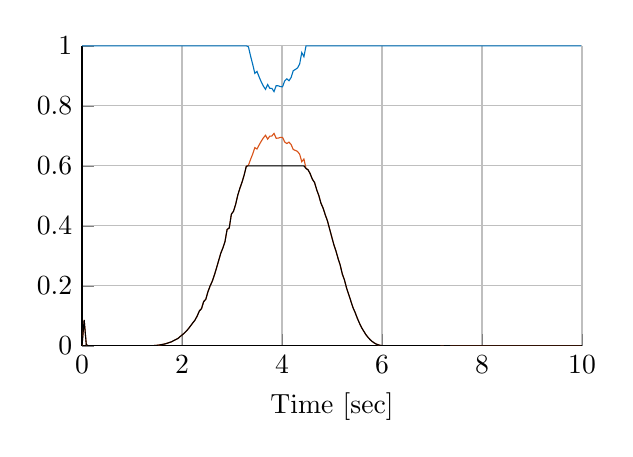
\begin{tikzpicture}

\begin{axis}[%
width=2.5in,
height=1.5in,
at={(0.758in,0.481in)},
scale only axis,
xmin=0,
xmax=10,
xlabel={Time [sec]},
xmajorgrids,
ymin=0,
ymax=1,
ymajorgrids,
axis background/.style={fill=white},
axis x line*=bottom,
axis y line*=left
]
\addplot [color=mycolor1,solid,forget plot]
  table[row sep=crcr]{%
0	1\\
0.0426666666666667	1\\
0.0853333333333333	1\\
0.128	1\\
0.170666666666667	1\\
0.213333333333333	1\\
0.256	1\\
0.298666666666667	1\\
0.341333333333333	1\\
0.384	1\\
0.426666666666667	1\\
0.469333333333333	1\\
0.512	1\\
0.554666666666667	1\\
0.597333333333333	1\\
0.64	1\\
0.682666666666667	1\\
0.725333333333333	1\\
0.768	1\\
0.810666666666667	1\\
0.853333333333333	1\\
0.896	1\\
0.938666666666667	1\\
0.981333333333333	1\\
1.024	1\\
1.06666666666667	1\\
1.10933333333333	1\\
1.152	1\\
1.19466666666667	1\\
1.23733333333333	1\\
1.28	1\\
1.32266666666667	1\\
1.36533333333333	1\\
1.408	1\\
1.45066666666667	1\\
1.49333333333333	1\\
1.536	1\\
1.57866666666667	1\\
1.62133333333333	1\\
1.664	1\\
1.70666666666667	1\\
1.74933333333333	1\\
1.792	1\\
1.83466666666667	1\\
1.87733333333333	1\\
1.92	1\\
1.96266666666667	1\\
2.00533333333333	1\\
2.048	1\\
2.09066666666667	1\\
2.13333333333333	1\\
2.176	1\\
2.21866666666667	1\\
2.26133333333333	1\\
2.304	1\\
2.34666666666667	1\\
2.38933333333333	1\\
2.432	1\\
2.47466666666667	1\\
2.51733333333333	1\\
2.56	1\\
2.60266666666667	1\\
2.64533333333333	1\\
2.688	1\\
2.73066666666667	1\\
2.77333333333333	1\\
2.816	1\\
2.85866666666667	1\\
2.90133333333333	1\\
2.944	1\\
2.98666666666667	1\\
3.02933333333333	1\\
3.072	1\\
3.11466666666667	1\\
3.15733333333333	1\\
3.2	1\\
3.24266666666667	1\\
3.28533333333333	1\\
3.328	0.996662151731393\\
3.37066666666667	0.965781467233386\\
3.41333333333333	0.93838961751612\\
3.456	0.908206081863302\\
3.49866666666667	0.914678909356829\\
3.54133333333333	0.896518433472737\\
3.584	0.879751367626536\\
3.62666666666667	0.865793725504439\\
3.66933333333333	0.854838303419917\\
3.712	0.870968515517342\\
3.75466666666667	0.858564925706032\\
3.79733333333333	0.85794920383526\\
3.84	0.847411869583181\\
3.88266666666667	0.867249658108438\\
3.92533333333333	0.866657595186744\\
3.968	0.863790850873918\\
4.01066666666667	0.863610256060327\\
4.05333333333333	0.883151245669426\\
4.096	0.889862071916161\\
4.13866666666667	0.883735364740767\\
4.18133333333333	0.894273747835014\\
4.224	0.917000963841052\\
4.26666666666667	0.921231673811068\\
4.30933333333333	0.92611974943379\\
4.352	0.939168136617217\\
4.39466666666667	0.977569606851807\\
4.43733333333333	0.963595357830717\\
4.48	1\\
4.52266666666667	1\\
4.56533333333333	1\\
4.608	1\\
4.65066666666667	1\\
4.69333333333333	1\\
4.736	1\\
4.77866666666667	1\\
4.82133333333333	1\\
4.864	1\\
4.90666666666667	1\\
4.94933333333333	1\\
4.992	1\\
5.03466666666667	1\\
5.07733333333333	1\\
5.12	1\\
5.16266666666667	1\\
5.20533333333333	1\\
5.248	1\\
5.29066666666667	1\\
5.33333333333333	1\\
5.376	1\\
5.41866666666667	1\\
5.46133333333333	1\\
5.504	1\\
5.54666666666667	1\\
5.58933333333333	1\\
5.632	1\\
5.67466666666667	1\\
5.71733333333333	1\\
5.76	1\\
5.80266666666667	1\\
5.84533333333333	1\\
5.888	1\\
5.93066666666667	1\\
5.97333333333333	1\\
6.016	1\\
6.05866666666667	1\\
6.10133333333333	1\\
6.144	1\\
6.18666666666667	1\\
6.22933333333333	1\\
6.272	1\\
6.31466666666667	1\\
6.35733333333333	1\\
6.4	1\\
6.44266666666667	1\\
6.48533333333333	1\\
6.528	1\\
6.57066666666667	1\\
6.61333333333333	1\\
6.656	1\\
6.69866666666667	1\\
6.74133333333333	1\\
6.784	1\\
6.82666666666667	1\\
6.86933333333333	1\\
6.912	1\\
6.95466666666667	1\\
6.99733333333333	1\\
7.04	1\\
7.08266666666667	1\\
7.12533333333333	1\\
7.168	1\\
7.21066666666667	1\\
7.25333333333333	1\\
7.296	1\\
7.33866666666667	1\\
7.38133333333333	1\\
7.424	1\\
7.46666666666667	1\\
7.50933333333333	1\\
7.552	1\\
7.59466666666667	1\\
7.63733333333333	1\\
7.68	1\\
7.72266666666667	1\\
7.76533333333333	1\\
7.808	1\\
7.85066666666667	1\\
7.89333333333333	1\\
7.936	1\\
7.97866666666667	1\\
8.02133333333333	1\\
8.064	1\\
8.10666666666667	1\\
8.14933333333333	1\\
8.192	1\\
8.23466666666667	1\\
8.27733333333333	1\\
8.32	1\\
8.36266666666667	1\\
8.40533333333333	1\\
8.448	1\\
8.49066666666667	1\\
8.53333333333333	1\\
8.576	1\\
8.61866666666667	1\\
8.66133333333333	1\\
8.704	1\\
8.74666666666667	1\\
8.78933333333333	1\\
8.832	1\\
8.87466666666667	1\\
8.91733333333333	1\\
8.96	1\\
9.00266666666667	1\\
9.04533333333333	1\\
9.088	1\\
9.13066666666667	1\\
9.17333333333333	1\\
9.216	1\\
9.25866666666667	1\\
9.30133333333333	1\\
9.344	1\\
9.38666666666667	1\\
9.42933333333333	1\\
9.472	1\\
9.51466666666667	1\\
9.55733333333333	1\\
9.6	1\\
9.64266666666667	1\\
9.68533333333333	1\\
9.728	1\\
9.77066666666667	1\\
9.81333333333333	1\\
9.856	1\\
9.89866666666667	1\\
9.94133333333333	1\\
9.984	1\\
};
\addplot [color=mycolor2,solid,forget plot]
  table[row sep=crcr]{%
0	0.000665310698843603\\
0.0426666666666667	0.0864776364105639\\
0.0853333333333333	0.00339967148176734\\
0.128	0.000223209352052432\\
0.170666666666667	0.000232409702435229\\
0.213333333333333	0.00024897169868072\\
0.256	0.000285801007016565\\
0.298666666666667	0.000297702524995538\\
0.341333333333333	0.000294934481278594\\
0.384	0.000296019488172937\\
0.426666666666667	0.000297164500352149\\
0.469333333333333	0.000290245296276126\\
0.512	0.000273067707096276\\
0.554666666666667	0.000246469482036333\\
0.597333333333333	0.000211376728394275\\
0.64	0.00016744198107956\\
0.682666666666667	0.000112411376694508\\
0.725333333333333	4.97985957362409e-05\\
0.768	5.21340270121921e-05\\
0.810666666666667	0.000116675315104569\\
0.853333333333333	0.000213056008264027\\
0.896	0.000307294780054194\\
0.938666666666667	0.0003818987800108\\
0.981333333333333	0.000512457285307295\\
1.024	0.000552551104803335\\
1.06666666666667	0.000680265305263416\\
1.10933333333333	0.000699998103580968\\
1.152	0.000736358903856387\\
1.19466666666667	0.000770021678873457\\
1.23733333333333	0.000698767797443855\\
1.28	0.00059193081276409\\
1.32266666666667	0.000459475335924129\\
1.36533333333333	0.000355436855584403\\
1.408	0.000527633015620785\\
1.45066666666667	0.000986551655156116\\
1.49333333333333	0.00163826585054485\\
1.536	0.00251046226546906\\
1.57866666666667	0.0037111574651577\\
1.62133333333333	0.00517052474986983\\
1.664	0.00654289503868774\\
1.70666666666667	0.00868845863057363\\
1.74933333333333	0.0113277350526885\\
1.792	0.0135259971142721\\
1.83466666666667	0.0175278406980728\\
1.87733333333333	0.0209804727364134\\
1.92	0.0247381674289943\\
1.96266666666667	0.0309310323096956\\
2.00533333333333	0.0367328689957315\\
2.048	0.0427055528098021\\
2.09066666666667	0.049855011725075\\
2.13333333333333	0.0582313148930913\\
2.176	0.0675626309055514\\
2.21866666666667	0.0770666881729873\\
2.26133333333333	0.0862980028544732\\
2.304	0.0997307166102876\\
2.34666666666667	0.116301865322749\\
2.38933333333333	0.123751791582908\\
2.432	0.147190933621082\\
2.47466666666667	0.155001843997694\\
2.51733333333333	0.179641914040256\\
2.56	0.198974522988724\\
2.60266666666667	0.214534530598528\\
2.64533333333333	0.235037027272627\\
2.688	0.258362813179426\\
2.73066666666667	0.283155307309969\\
2.77333333333333	0.307774625774315\\
2.816	0.325914018147003\\
2.85866666666667	0.347230472421214\\
2.90133333333333	0.387810824368077\\
2.944	0.392878826522048\\
2.98666666666667	0.438775248189825\\
3.02933333333333	0.448426045304505\\
3.072	0.471481509577598\\
3.11466666666667	0.50211430566478\\
3.15733333333333	0.5253631588727\\
3.2	0.545503929000724\\
3.24266666666667	0.569426814983639\\
3.28533333333333	0.59852881353414\\
3.328	0.602009416087172\\
3.37066666666667	0.621258556264061\\
3.41333333333333	0.639393263523286\\
3.456	0.660643010415679\\
3.49866666666667	0.655967896342881\\
3.54133333333333	0.669255619960709\\
3.584	0.682010874980198\\
3.62666666666667	0.693005715247499\\
3.66933333333333	0.701887126020914\\
3.712	0.688888277027568\\
3.75466666666667	0.698840567597839\\
3.79733333333333	0.699342102443643\\
3.84	0.708038229739599\\
3.88266666666667	0.691842302144763\\
3.92533333333333	0.692314938832001\\
3.968	0.694612589833483\\
4.01066666666667	0.69475784451324\\
4.05333333333333	0.679385329457586\\
4.096	0.674261797345746\\
4.13866666666667	0.678936278821435\\
4.18133333333333	0.67093549536992\\
4.224	0.654306836807208\\
4.26666666666667	0.65130196568019\\
4.30933333333333	0.647864382944891\\
4.352	0.638863241422495\\
4.39466666666667	0.61376703591702\\
4.43733333333333	0.622668005946752\\
4.48	0.590998290564149\\
4.52266666666667	0.586340978510395\\
4.56533333333333	0.572541390249848\\
4.608	0.554802187556847\\
4.65066666666667	0.544106920953253\\
4.69333333333333	0.520172744056389\\
4.736	0.500632951146593\\
4.77866666666667	0.475098051728122\\
4.82133333333333	0.459153213226307\\
4.864	0.436763608738208\\
4.90666666666667	0.417413044677455\\
4.94933333333333	0.390799497970971\\
4.992	0.364258123039305\\
5.03466666666667	0.338187441405853\\
5.07733333333333	0.316580754252238\\
5.12	0.291423140738191\\
5.16266666666667	0.269429329267443\\
5.20533333333333	0.23943286784774\\
5.248	0.219677213775725\\
5.29066666666667	0.192738105848834\\
5.33333333333333	0.171182023909518\\
5.376	0.149291646464307\\
5.41866666666667	0.127363203875613\\
5.46133333333333	0.111296528790569\\
5.504	0.0926488162167592\\
5.54666666666667	0.0761026975854887\\
5.58933333333333	0.0612538533180002\\
5.632	0.0493616838539349\\
5.67466666666667	0.037859023228239\\
5.71733333333333	0.0288357490648459\\
5.76	0.0207546898017366\\
5.80266666666667	0.0145204642515098\\
5.84533333333333	0.00935227374079\\
5.888	0.00563318871632384\\
5.93066666666667	0.00286605427260342\\
5.97333333333333	0.00112853455704289\\
6.016	0.000457151904659207\\
6.05866666666667	0.000693745967030103\\
6.10133333333333	0.000772090948849886\\
6.144	0.000629512419675635\\
6.18666666666667	0.000349162656028732\\
6.22933333333333	9.87940972823937e-05\\
6.272	0.000254969646945357\\
6.31466666666667	0.000426510582542647\\
6.35733333333333	0.000519036575055806\\
6.4	0.000491511105292594\\
6.44266666666667	0.000399445616667678\\
6.48533333333333	0.000246782061413681\\
6.528	8.01509993499446e-05\\
6.57066666666667	0.000110783692934738\\
6.61333333333333	0.000235961757680276\\
6.656	0.000304238474918873\\
6.69866666666667	0.000324939120442809\\
6.74133333333333	0.000280196875921051\\
6.784	0.000200089851325884\\
6.82666666666667	0.000102898945233571\\
6.86933333333333	3.09934345839719e-05\\
6.912	0.000101098090857212\\
6.95466666666667	0.000157389979039587\\
6.99733333333333	0.000180763079664465\\
7.04	0.000169822606097089\\
7.08266666666667	0.000133211080715111\\
7.12533333333333	8.19143961552846e-05\\
7.168	3.09158584497086e-05\\
7.21066666666667	2.10113447670854e-05\\
7.25333333333333	4.49286648484074e-05\\
7.296	5.42093988088787e-05\\
7.33866666666667	4.4157895064341e-05\\
7.38133333333333	2.76859676738284e-05\\
7.424	7.91239327228418e-06\\
7.46666666666667	1.45712277505793e-05\\
7.50933333333333	2.38657345077776e-05\\
7.552	2.79018837746144e-05\\
7.59466666666667	2.22380097274004e-05\\
7.63733333333333	1.43401425319648e-05\\
7.68	6.27648901767715e-06\\
7.72266666666667	2.4148137675687e-06\\
7.76533333333333	3.88947611625917e-06\\
7.808	4.60596474014671e-06\\
7.85066666666667	2.28487995059953e-06\\
7.89333333333333	1.32062306387396e-06\\
7.936	2.48601828740123e-07\\
7.97866666666667	1.19577887704704e-06\\
8.02133333333333	8.21985036600566e-07\\
8.064	4.60752634284164e-07\\
8.10666666666667	1.25003399807337e-07\\
8.14933333333333	5.57314870274513e-08\\
8.192	8.03322039481693e-08\\
8.23466666666667	1.59454974097026e-07\\
8.27733333333333	1.67064145636944e-07\\
8.32	9.89712453571405e-08\\
8.36266666666667	3.35962278056592e-08\\
8.40533333333333	1.30867386741705e-08\\
8.448	1.63616468639176e-08\\
8.49066666666667	2.84748709621327e-08\\
8.53333333333333	1.65686860840004e-08\\
8.576	1.87247454123607e-08\\
8.61866666666667	3.30568249736066e-08\\
8.66133333333333	2.15973037805438e-08\\
8.704	7.70096646256557e-09\\
8.74666666666667	1.50963983011663e-08\\
8.78933333333333	8.12958458458862e-09\\
8.832	6.02153112560425e-09\\
8.87466666666667	6.09455537430122e-09\\
8.91733333333333	4.24091784693298e-09\\
8.96	8.17862016119566e-09\\
9.00266666666667	3.94373254148258e-09\\
9.04533333333333	3.76469486832534e-09\\
9.088	4.52646995316457e-09\\
9.13066666666667	1.50964267700306e-08\\
9.17333333333333	1.97701371402558e-08\\
9.216	1.2368015443575e-08\\
9.25866666666667	3.85186349133356e-09\\
9.30133333333333	5.61836143233769e-09\\
9.344	2.0728335719488e-09\\
9.38666666666667	4.01173323997444e-09\\
9.42933333333333	2.07404045260869e-09\\
9.472	3.11766156635754e-09\\
9.51466666666667	3.14654451914122e-09\\
9.55733333333333	1.11720125030847e-09\\
9.6	7.71963304837536e-10\\
9.64266666666667	1.69571998331782e-09\\
9.68533333333333	1.26604206811313e-09\\
9.728	5.35014629699236e-10\\
9.77066666666667	4.75402997466168e-10\\
9.81333333333333	1.25797055358132e-10\\
9.856	1.45775928697891e-11\\
9.89866666666667	9.77160384802232e-13\\
9.94133333333333	1.19437816673104e-13\\
9.984	9.56370724067793e-09\\
};
\addplot [color=mycolor3,solid,forget plot]
  table[row sep=crcr]{%
0	0.000665310698843603\\
0.0426666666666667	0.0864776364105639\\
0.0853333333333333	0.00339967148176734\\
0.128	0.000223209352052432\\
0.170666666666667	0.000232409702435229\\
0.213333333333333	0.00024897169868072\\
0.256	0.000285801007016565\\
0.298666666666667	0.000297702524995538\\
0.341333333333333	0.000294934481278594\\
0.384	0.000296019488172937\\
0.426666666666667	0.000297164500352149\\
0.469333333333333	0.000290245296276126\\
0.512	0.000273067707096276\\
0.554666666666667	0.000246469482036333\\
0.597333333333333	0.000211376728394275\\
0.64	0.00016744198107956\\
0.682666666666667	0.000112411376694508\\
0.725333333333333	4.97985957362409e-05\\
0.768	5.21340270121921e-05\\
0.810666666666667	0.000116675315104569\\
0.853333333333333	0.000213056008264027\\
0.896	0.000307294780054194\\
0.938666666666667	0.0003818987800108\\
0.981333333333333	0.000512457285307295\\
1.024	0.000552551104803335\\
1.06666666666667	0.000680265305263416\\
1.10933333333333	0.000699998103580968\\
1.152	0.000736358903856387\\
1.19466666666667	0.000770021678873457\\
1.23733333333333	0.000698767797443855\\
1.28	0.00059193081276409\\
1.32266666666667	0.000459475335924129\\
1.36533333333333	0.000355436855584403\\
1.408	0.000527633015620785\\
1.45066666666667	0.000986551655156116\\
1.49333333333333	0.00163826585054485\\
1.536	0.00251046226546906\\
1.57866666666667	0.0037111574651577\\
1.62133333333333	0.00517052474986983\\
1.664	0.00654289503868774\\
1.70666666666667	0.00868845863057363\\
1.74933333333333	0.0113277350526885\\
1.792	0.0135259971142721\\
1.83466666666667	0.0175278406980728\\
1.87733333333333	0.0209804727364134\\
1.92	0.0247381674289943\\
1.96266666666667	0.0309310323096956\\
2.00533333333333	0.0367328689957315\\
2.048	0.0427055528098021\\
2.09066666666667	0.049855011725075\\
2.13333333333333	0.0582313148930913\\
2.176	0.0675626309055514\\
2.21866666666667	0.0770666881729873\\
2.26133333333333	0.0862980028544732\\
2.304	0.0997307166102876\\
2.34666666666667	0.116301865322749\\
2.38933333333333	0.123751791582908\\
2.432	0.147190933621082\\
2.47466666666667	0.155001843997694\\
2.51733333333333	0.179641914040256\\
2.56	0.198974522988724\\
2.60266666666667	0.214534530598528\\
2.64533333333333	0.235037027272627\\
2.688	0.258362813179426\\
2.73066666666667	0.283155307309969\\
2.77333333333333	0.307774625774315\\
2.816	0.325914018147003\\
2.85866666666667	0.347230472421214\\
2.90133333333333	0.387810824368077\\
2.944	0.392878826522048\\
2.98666666666667	0.438775248189825\\
3.02933333333333	0.448426045304505\\
3.072	0.471481509577598\\
3.11466666666667	0.50211430566478\\
3.15733333333333	0.5253631588727\\
3.2	0.545503929000724\\
3.24266666666667	0.569426814983639\\
3.28533333333333	0.59852881353414\\
3.328	0.6\\
3.37066666666667	0.6\\
3.41333333333333	0.6\\
3.456	0.6\\
3.49866666666667	0.6\\
3.54133333333333	0.6\\
3.584	0.6\\
3.62666666666667	0.6\\
3.66933333333333	0.6\\
3.712	0.6\\
3.75466666666667	0.6\\
3.79733333333333	0.6\\
3.84	0.6\\
3.88266666666667	0.6\\
3.92533333333333	0.6\\
3.968	0.6\\
4.01066666666667	0.6\\
4.05333333333333	0.6\\
4.096	0.6\\
4.13866666666667	0.6\\
4.18133333333333	0.6\\
4.224	0.6\\
4.26666666666667	0.6\\
4.30933333333333	0.6\\
4.352	0.6\\
4.39466666666667	0.6\\
4.43733333333333	0.6\\
4.48	0.590998290564149\\
4.52266666666667	0.586340978510395\\
4.56533333333333	0.572541390249848\\
4.608	0.554802187556847\\
4.65066666666667	0.544106920953253\\
4.69333333333333	0.520172744056389\\
4.736	0.500632951146593\\
4.77866666666667	0.475098051728122\\
4.82133333333333	0.459153213226307\\
4.864	0.436763608738208\\
4.90666666666667	0.417413044677455\\
4.94933333333333	0.390799497970971\\
4.992	0.364258123039305\\
5.03466666666667	0.338187441405853\\
5.07733333333333	0.316580754252238\\
5.12	0.291423140738191\\
5.16266666666667	0.269429329267443\\
5.20533333333333	0.23943286784774\\
5.248	0.219677213775725\\
5.29066666666667	0.192738105848834\\
5.33333333333333	0.171182023909518\\
5.376	0.149291646464307\\
5.41866666666667	0.127363203875613\\
5.46133333333333	0.111296528790569\\
5.504	0.0926488162167592\\
5.54666666666667	0.0761026975854887\\
5.58933333333333	0.0612538533180002\\
5.632	0.0493616838539349\\
5.67466666666667	0.037859023228239\\
5.71733333333333	0.0288357490648459\\
5.76	0.0207546898017366\\
5.80266666666667	0.0145204642515098\\
5.84533333333333	0.00935227374079\\
5.888	0.00563318871632384\\
5.93066666666667	0.00286605427260342\\
5.97333333333333	0.00112853455704289\\
6.016	0.000457151904659207\\
6.05866666666667	0.000693745967030103\\
6.10133333333333	0.000772090948849886\\
6.144	0.000629512419675635\\
6.18666666666667	0.000349162656028732\\
6.22933333333333	9.87940972823937e-05\\
6.272	0.000254969646945357\\
6.31466666666667	0.000426510582542647\\
6.35733333333333	0.000519036575055806\\
6.4	0.000491511105292594\\
6.44266666666667	0.000399445616667678\\
6.48533333333333	0.000246782061413681\\
6.528	8.01509993499446e-05\\
6.57066666666667	0.000110783692934738\\
6.61333333333333	0.000235961757680276\\
6.656	0.000304238474918873\\
6.69866666666667	0.000324939120442809\\
6.74133333333333	0.000280196875921051\\
6.784	0.000200089851325884\\
6.82666666666667	0.000102898945233571\\
6.86933333333333	3.09934345839719e-05\\
6.912	0.000101098090857212\\
6.95466666666667	0.000157389979039587\\
6.99733333333333	0.000180763079664465\\
7.04	0.000169822606097089\\
7.08266666666667	0.000133211080715111\\
7.12533333333333	8.19143961552846e-05\\
7.168	3.09158584497086e-05\\
7.21066666666667	2.10113447670854e-05\\
7.25333333333333	4.49286648484074e-05\\
7.296	5.42093988088787e-05\\
7.33866666666667	4.4157895064341e-05\\
7.38133333333333	2.76859676738284e-05\\
7.424	7.91239327228418e-06\\
7.46666666666667	1.45712277505793e-05\\
7.50933333333333	2.38657345077776e-05\\
7.552	2.79018837746144e-05\\
7.59466666666667	2.22380097274004e-05\\
7.63733333333333	1.43401425319648e-05\\
7.68	6.27648901767715e-06\\
7.72266666666667	2.4148137675687e-06\\
7.76533333333333	3.88947611625917e-06\\
7.808	4.60596474014671e-06\\
7.85066666666667	2.28487995059953e-06\\
7.89333333333333	1.32062306387396e-06\\
7.936	2.48601828740123e-07\\
7.97866666666667	1.19577887704704e-06\\
8.02133333333333	8.21985036600566e-07\\
8.064	4.60752634284164e-07\\
8.10666666666667	1.25003399807337e-07\\
8.14933333333333	5.57314870274513e-08\\
8.192	8.03322039481693e-08\\
8.23466666666667	1.59454974097026e-07\\
8.27733333333333	1.67064145636944e-07\\
8.32	9.89712453571405e-08\\
8.36266666666667	3.35962278056592e-08\\
8.40533333333333	1.30867386741705e-08\\
8.448	1.63616468639176e-08\\
8.49066666666667	2.84748709621327e-08\\
8.53333333333333	1.65686860840004e-08\\
8.576	1.87247454123607e-08\\
8.61866666666667	3.30568249736066e-08\\
8.66133333333333	2.15973037805438e-08\\
8.704	7.70096646256557e-09\\
8.74666666666667	1.50963983011663e-08\\
8.78933333333333	8.12958458458862e-09\\
8.832	6.02153112560425e-09\\
8.87466666666667	6.09455537430122e-09\\
8.91733333333333	4.24091784693298e-09\\
8.96	8.17862016119566e-09\\
9.00266666666667	3.94373254148258e-09\\
9.04533333333333	3.76469486832534e-09\\
9.088	4.52646995316457e-09\\
9.13066666666667	1.50964267700306e-08\\
9.17333333333333	1.97701371402558e-08\\
9.216	1.2368015443575e-08\\
9.25866666666667	3.85186349133356e-09\\
9.30133333333333	5.61836143233769e-09\\
9.344	2.0728335719488e-09\\
9.38666666666667	4.01173323997444e-09\\
9.42933333333333	2.07404045260869e-09\\
9.472	3.11766156635754e-09\\
9.51466666666667	3.14654451914122e-09\\
9.55733333333333	1.11720125030847e-09\\
9.6	7.71963304837536e-10\\
9.64266666666667	1.69571998331782e-09\\
9.68533333333333	1.26604206811313e-09\\
9.728	5.35014629699236e-10\\
9.77066666666667	4.75402997466168e-10\\
9.81333333333333	1.25797055358132e-10\\
9.856	1.45775928697891e-11\\
9.89866666666667	9.77160384802232e-13\\
9.94133333333333	1.19437816673104e-13\\
9.984	9.56370724067793e-09\\
};
\end{axis}
\end{tikzpicture}%
    \caption{Band 2 from 66 Hz to 132 Hz}
    \label{fig:Band2Simulation}
\end{subfigure}
\begin{subfigure}[t]{0.49\textwidth}
    \centering
    \tikzsetnextfilename{Band3Simulation}
    % This file was created by matlab2tikz.
%
%The latest updates can be retrieved from
%  http://www.mathworks.com/matlabcentral/fileexchange/22022-matlab2tikz-matlab2tikz
%where you can also make suggestions and rate matlab2tikz.
%
\definecolor{mycolor1}{rgb}{0.00000,0.44700,0.74100}%
\definecolor{mycolor2}{rgb}{0.85000,0.32500,0.09800}%
\definecolor{mycolor3}{rgb}{0.00,0.00,0.00}%
%
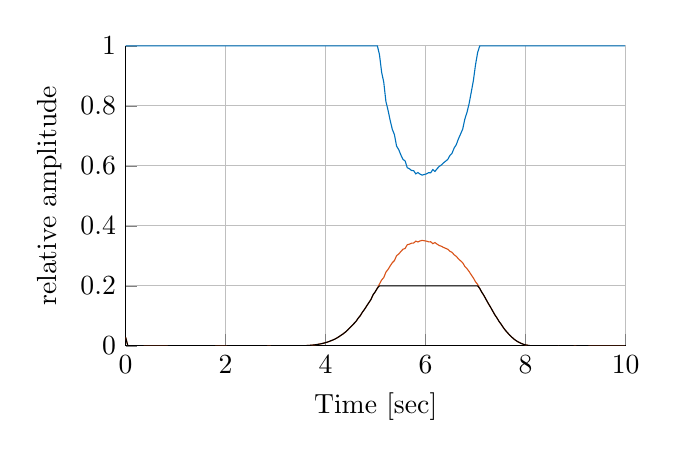
\begin{tikzpicture}

\begin{axis}[%
width=2.5in,
height=1.5in,
at={(0.758in,0.481in)},
scale only axis,
xmin=0,
xmax=10,
xlabel={Time [sec]},
xmajorgrids,
ymin=0,
ymax=1,
ylabel={relative amplitude},
ymajorgrids,
axis background/.style={fill=white},
axis x line*=bottom,
axis y line*=left
]
\addplot [color=mycolor1,solid,forget plot]
  table[row sep=crcr]{%
0	1\\
0.0426666666666667	1\\
0.0853333333333333	1\\
0.128	1\\
0.170666666666667	1\\
0.213333333333333	1\\
0.256	1\\
0.298666666666667	1\\
0.341333333333333	1\\
0.384	1\\
0.426666666666667	1\\
0.469333333333333	1\\
0.512	1\\
0.554666666666667	1\\
0.597333333333333	1\\
0.64	1\\
0.682666666666667	1\\
0.725333333333333	1\\
0.768	1\\
0.810666666666667	1\\
0.853333333333333	1\\
0.896	1\\
0.938666666666667	1\\
0.981333333333333	1\\
1.024	1\\
1.06666666666667	1\\
1.10933333333333	1\\
1.152	1\\
1.19466666666667	1\\
1.23733333333333	1\\
1.28	1\\
1.32266666666667	1\\
1.36533333333333	1\\
1.408	1\\
1.45066666666667	1\\
1.49333333333333	1\\
1.536	1\\
1.57866666666667	1\\
1.62133333333333	1\\
1.664	1\\
1.70666666666667	1\\
1.74933333333333	1\\
1.792	1\\
1.83466666666667	1\\
1.87733333333333	1\\
1.92	1\\
1.96266666666667	1\\
2.00533333333333	1\\
2.048	1\\
2.09066666666667	1\\
2.13333333333333	1\\
2.176	1\\
2.21866666666667	1\\
2.26133333333333	1\\
2.304	1\\
2.34666666666667	1\\
2.38933333333333	1\\
2.432	1\\
2.47466666666667	1\\
2.51733333333333	1\\
2.56	1\\
2.60266666666667	1\\
2.64533333333333	1\\
2.688	1\\
2.73066666666667	1\\
2.77333333333333	1\\
2.816	1\\
2.85866666666667	1\\
2.90133333333333	1\\
2.944	1\\
2.98666666666667	1\\
3.02933333333333	1\\
3.072	1\\
3.11466666666667	1\\
3.15733333333333	1\\
3.2	1\\
3.24266666666667	1\\
3.28533333333333	1\\
3.328	1\\
3.37066666666667	1\\
3.41333333333333	1\\
3.456	1\\
3.49866666666667	1\\
3.54133333333333	1\\
3.584	1\\
3.62666666666667	1\\
3.66933333333333	1\\
3.712	1\\
3.75466666666667	1\\
3.79733333333333	1\\
3.84	1\\
3.88266666666667	1\\
3.92533333333333	1\\
3.968	1\\
4.01066666666667	1\\
4.05333333333333	1\\
4.096	1\\
4.13866666666667	1\\
4.18133333333333	1\\
4.224	1\\
4.26666666666667	1\\
4.30933333333333	1\\
4.352	1\\
4.39466666666667	1\\
4.43733333333333	1\\
4.48	1\\
4.52266666666667	1\\
4.56533333333333	1\\
4.608	1\\
4.65066666666667	1\\
4.69333333333333	1\\
4.736	1\\
4.77866666666667	1\\
4.82133333333333	1\\
4.864	1\\
4.90666666666667	1\\
4.94933333333333	1\\
4.992	1\\
5.03466666666667	1\\
5.07733333333333	0.969880895980676\\
5.12	0.911709109696262\\
5.16266666666667	0.878566467045722\\
5.20533333333333	0.814684493807506\\
5.248	0.785362677451813\\
5.29066666666667	0.751385749497003\\
5.33333333333333	0.721769712703029\\
5.376	0.703640095623825\\
5.41866666666667	0.665847928629747\\
5.46133333333333	0.653946895360279\\
5.504	0.636420973537659\\
5.54666666666667	0.62121444677337\\
5.58933333333333	0.616347616719769\\
5.632	0.593789349850404\\
5.67466666666667	0.590311243223664\\
5.71733333333333	0.584503563699738\\
5.76	0.583871006663183\\
5.80266666666667	0.573174411309484\\
5.84533333333333	0.57762560767088\\
5.888	0.57223745755078\\
5.93066666666667	0.569074867692195\\
5.97333333333333	0.57105948822274\\
6.016	0.573066329461291\\
6.05866666666667	0.577110692498977\\
6.10133333333333	0.576760788197133\\
6.144	0.587394551662804\\
6.18666666666667	0.581267747476056\\
6.22933333333333	0.590269236135185\\
6.272	0.5982441738293\\
6.31466666666667	0.602738125651154\\
6.35733333333333	0.609779080921584\\
6.4	0.615461509713572\\
6.44266666666667	0.621351925592731\\
6.48533333333333	0.634259959142679\\
6.528	0.641876946247208\\
6.57066666666667	0.659518915310653\\
6.61333333333333	0.670547977484076\\
6.656	0.690059430798031\\
6.69866666666667	0.705887652442372\\
6.74133333333333	0.722388896704544\\
6.784	0.755932365552911\\
6.82666666666667	0.777977236375048\\
6.86933333333333	0.807285608013932\\
6.912	0.84520528220781\\
6.95466666666667	0.883876215146974\\
6.99733333333333	0.936482506162066\\
7.04	0.977712900587785\\
7.08266666666667	1\\
7.12533333333333	1\\
7.168	1\\
7.21066666666667	1\\
7.25333333333333	1\\
7.296	1\\
7.33866666666667	1\\
7.38133333333333	1\\
7.424	1\\
7.46666666666667	1\\
7.50933333333333	1\\
7.552	1\\
7.59466666666667	1\\
7.63733333333333	1\\
7.68	1\\
7.72266666666667	1\\
7.76533333333333	1\\
7.808	1\\
7.85066666666667	1\\
7.89333333333333	1\\
7.936	1\\
7.97866666666667	1\\
8.02133333333333	1\\
8.064	1\\
8.10666666666667	1\\
8.14933333333333	1\\
8.192	1\\
8.23466666666667	1\\
8.27733333333333	1\\
8.32	1\\
8.36266666666667	1\\
8.40533333333333	1\\
8.448	1\\
8.49066666666667	1\\
8.53333333333333	1\\
8.576	1\\
8.61866666666667	1\\
8.66133333333333	1\\
8.704	1\\
8.74666666666667	1\\
8.78933333333333	1\\
8.832	1\\
8.87466666666667	1\\
8.91733333333333	1\\
8.96	1\\
9.00266666666667	1\\
9.04533333333333	1\\
9.088	1\\
9.13066666666667	1\\
9.17333333333333	1\\
9.216	1\\
9.25866666666667	1\\
9.30133333333333	1\\
9.344	1\\
9.38666666666667	1\\
9.42933333333333	1\\
9.472	1\\
9.51466666666667	1\\
9.55733333333333	1\\
9.6	1\\
9.64266666666667	1\\
9.68533333333333	1\\
9.728	1\\
9.77066666666667	1\\
9.81333333333333	1\\
9.856	1\\
9.89866666666667	1\\
9.94133333333333	1\\
9.984	1\\
};
\addplot [color=mycolor2,solid,forget plot]
  table[row sep=crcr]{%
0	0.0282388040914952\\
0.0426666666666667	0.00107177953713978\\
0.0853333333333333	6.28322277133213e-05\\
0.128	6.49665856522593e-05\\
0.170666666666667	5.83868464472985e-05\\
0.213333333333333	5.08043003298312e-05\\
0.256	4.8447819329928e-05\\
0.298666666666667	4.44035819191288e-05\\
0.341333333333333	3.80201251988048e-05\\
0.384	3.15835569119565e-05\\
0.426666666666667	2.5695117576987e-05\\
0.469333333333333	1.99291890458e-05\\
0.512	1.39791291213467e-05\\
0.554666666666667	7.82340422532203e-06\\
0.597333333333333	2.20267674432613e-06\\
0.64	5.60656592377416e-06\\
0.682666666666667	1.14465812196147e-05\\
0.725333333333333	1.75207609088655e-05\\
0.768	2.50073515752096e-05\\
0.810666666666667	3.15048709393531e-05\\
0.853333333333333	3.53812050205405e-05\\
0.896	4.44403352882454e-05\\
0.938666666666667	4.80572456386141e-05\\
0.981333333333333	5.49958930516467e-05\\
1.024	5.8693480592249e-05\\
1.06666666666667	6.65131238276677e-05\\
1.10933333333333	6.61668485200097e-05\\
1.152	7.4041098114331e-05\\
1.19466666666667	7.80128851625685e-05\\
1.23733333333333	7.79403771648501e-05\\
1.28	7.94514346383498e-05\\
1.32266666666667	8.16230669727775e-05\\
1.36533333333333	8.26930397306177e-05\\
1.408	8.25229662096235e-05\\
1.45066666666667	8.15572060212458e-05\\
1.49333333333333	8.00416880344101e-05\\
1.536	7.71229284329365e-05\\
1.57866666666667	7.10465500759938e-05\\
1.62133333333333	6.43786247550614e-05\\
1.664	6.14024124341161e-05\\
1.70666666666667	5.22368110766006e-05\\
1.74933333333333	4.37160267878224e-05\\
1.792	3.47885808489743e-05\\
1.83466666666667	2.43032850853508e-05\\
1.87733333333333	1.26683506611189e-05\\
1.92	4.1347904167323e-06\\
1.96266666666667	1.38811607553244e-05\\
2.00533333333333	2.70409226730704e-05\\
2.048	4.07477350060181e-05\\
2.09066666666667	5.51389976683688e-05\\
2.13333333333333	6.98742071387533e-05\\
2.176	8.39647245982223e-05\\
2.21866666666667	9.57893935574026e-05\\
2.26133333333333	0.000108008190704394\\
2.304	0.000124763982117828\\
2.34666666666667	0.000129926160047441\\
2.38933333333333	0.000142138694949415\\
2.432	0.000144383738049175\\
2.47466666666667	0.000154316188525305\\
2.51733333333333	0.000149807323013747\\
2.56	0.000146600138013003\\
2.60266666666667	0.000142080808307791\\
2.64533333333333	0.000132051652374333\\
2.688	0.000117196748859266\\
2.73066666666667	9.82715692625955e-05\\
2.77333333333333	7.39593894762916e-05\\
2.816	4.34154052307768e-05\\
2.85866666666667	1.53033162143408e-05\\
2.90133333333333	3.33900286447377e-05\\
2.944	7.19208638780501e-05\\
2.98666666666667	0.000117360017831419\\
3.02933333333333	0.000167502865755585\\
3.072	0.00021345172886878\\
3.11466666666667	0.000258489780014376\\
3.15733333333333	0.000301001091552116\\
3.2	0.000334583831176306\\
3.24266666666667	0.00035377318834095\\
3.28533333333333	0.000370780497753704\\
3.328	0.000362265970105241\\
3.37066666666667	0.000321808686669682\\
3.41333333333333	0.000257397854317076\\
3.456	0.000163432124308274\\
3.49866666666667	0.00010493639872278\\
3.54133333333333	0.00027837531450186\\
3.584	0.000569112006237081\\
3.62666666666667	0.00094179447150661\\
3.66933333333333	0.00139524665768068\\
3.712	0.00205280604485173\\
3.75466666666667	0.00270005842820592\\
3.79733333333333	0.00369313134035538\\
3.84	0.00471216072352423\\
3.88266666666667	0.00593604378290063\\
3.92533333333333	0.00744733009468972\\
3.968	0.00921865529945331\\
4.01066666666667	0.0110687949817519\\
4.05333333333333	0.0133425132124141\\
4.096	0.0161953321181614\\
4.13866666666667	0.019068251958538\\
4.18133333333333	0.0221536157989619\\
4.224	0.0260460561497728\\
4.26666666666667	0.0303783140689522\\
4.30933333333333	0.0353854672964277\\
4.352	0.040129705882825\\
4.39466666666667	0.0456700149383858\\
4.43733333333333	0.0519624846596325\\
4.48	0.0594291720956924\\
4.52266666666667	0.0663835854317335\\
4.56533333333333	0.0739714738832096\\
4.608	0.0816703690843484\\
4.65066666666667	0.092165494523071\\
4.69333333333333	0.10053368445218\\
4.736	0.112392639964266\\
4.77866666666667	0.12185934165038\\
4.82133333333333	0.133037567077694\\
4.864	0.143898535505801\\
4.90666666666667	0.154518592404813\\
4.94933333333333	0.170258741912115\\
4.992	0.18007163495179\\
5.03466666666667	0.192233681808087\\
5.07733333333333	0.206210887160298\\
5.12	0.21936821500734\\
5.16266666666667	0.227643561986292\\
5.20533333333333	0.245493809591589\\
5.248	0.254659414996546\\
5.29066666666667	0.266174864420686\\
5.33333333333333	0.277096692310626\\
5.376	0.284236218549607\\
5.41866666666667	0.300368885147066\\
5.46133333333333	0.305835231299346\\
5.504	0.314257399293842\\
5.54666666666667	0.3219500142645\\
5.58933333333333	0.324492209549555\\
5.632	0.336819783060082\\
5.67466666666667	0.338804321103235\\
5.71733333333333	0.342170711045897\\
5.76	0.342541413630038\\
5.80266666666667	0.348933930150644\\
5.84533333333333	0.34624503717286\\
5.888	0.349505257583128\\
5.93066666666667	0.351447606201751\\
5.97333333333333	0.350226209571341\\
6.016	0.34899974002662\\
6.05866666666667	0.34655396720163\\
6.10133333333333	0.346764211598312\\
6.144	0.340486644681735\\
6.18666666666667	0.344075515747136\\
6.22933333333333	0.338828432444674\\
6.272	0.33431165525578\\
6.31466666666667	0.331819062854095\\
6.35733333333333	0.327987637256647\\
6.4	0.324959395256216\\
6.44266666666667	0.321878780385548\\
6.48533333333333	0.31532811919948\\
6.528	0.311586202260913\\
6.57066666666667	0.303251347849203\\
6.61333333333333	0.298263519860888\\
6.656	0.289830108935265\\
6.69866666666667	0.283331206188407\\
6.74133333333333	0.276859183346224\\
6.784	0.264573934274813\\
6.82666666666667	0.2570769305949\\
6.86933333333333	0.247743794779193\\
6.912	0.236628904492372\\
6.95466666666667	0.226276028897037\\
6.99733333333333	0.213565121274554\\
7.04	0.204559027378859\\
7.08266666666667	0.190986141168696\\
7.12533333333333	0.177952965165217\\
7.168	0.167052723635734\\
7.21066666666667	0.153853650034617\\
7.25333333333333	0.14119957383787\\
7.296	0.129314946925276\\
7.33866666666667	0.116792180043506\\
7.38133333333333	0.104022796329725\\
7.424	0.0935720561119066\\
7.46666666666667	0.0817486653016014\\
7.50933333333333	0.0719462298941643\\
7.552	0.0613382177620069\\
7.59466666666667	0.0517093229525832\\
7.63733333333333	0.0437403911100275\\
7.68	0.0356634185925986\\
7.72266666666667	0.0290396483683797\\
7.76533333333333	0.0226625954420665\\
7.808	0.0173429881341511\\
7.85066666666667	0.0129737136653792\\
7.89333333333333	0.00933552195306145\\
7.936	0.00626687344467878\\
7.97866666666667	0.00401320845815973\\
8.02133333333333	0.00227144925075129\\
8.064	0.00109583422209982\\
8.10666666666667	0.000336848341113091\\
8.14933333333333	0.000208654209436348\\
8.192	0.000358722364832184\\
8.23466666666667	0.00036549952567879\\
8.27733333333333	0.000271047729289022\\
8.32	0.000126254108709634\\
8.36266666666667	5.32340484034458e-05\\
8.40533333333333	0.000159649302908678\\
8.448	0.000232921522390117\\
8.49066666666667	0.000260046192551051\\
8.53333333333333	0.000234648305506217\\
8.576	0.000177093136625545\\
8.61866666666667	9.47816288826688e-05\\
8.66133333333333	2.49057269214853e-05\\
8.704	7.68591810786823e-05\\
8.74666666666667	0.00013233902313696\\
8.78933333333333	0.00015890345262837\\
8.832	0.000156857430637336\\
8.87466666666667	0.000129353824636095\\
8.91733333333333	8.52921055010737e-05\\
8.96	3.43793428498935e-05\\
9.00266666666667	2.4889489579921e-05\\
9.04533333333333	6.17941486169677e-05\\
9.088	8.37425720058614e-05\\
9.13066666666667	9.0693920244702e-05\\
9.17333333333333	7.96989621737035e-05\\
9.216	5.89861727917862e-05\\
9.25866666666667	3.17558913632554e-05\\
9.30133333333333	8.83733243099352e-06\\
9.344	1.51632412940633e-05\\
9.38666666666667	2.46696918983858e-05\\
9.42933333333333	2.58749399363198e-05\\
9.472	2.01244793422252e-05\\
9.51466666666667	1.00209650363962e-05\\
9.55733333333333	3.13749655473897e-06\\
9.6	9.32927812226036e-06\\
9.64266666666667	1.30573615888476e-05\\
9.68533333333333	1.28916380400308e-05\\
9.728	1.02917884950535e-05\\
9.77066666666667	5.75639553993091e-06\\
9.81333333333333	1.77821806118978e-06\\
9.856	1.39707160523351e-06\\
9.89866666666667	2.12896345007753e-06\\
9.94133333333333	2.00120638913694e-06\\
9.984	1.37552429553707e-05\\
};
\addplot [color=mycolor3,solid,forget plot]
  table[row sep=crcr]{%
0	0.0282388040914952\\
0.0426666666666667	0.00107177953713978\\
0.0853333333333333	6.28322277133213e-05\\
0.128	6.49665856522593e-05\\
0.170666666666667	5.83868464472985e-05\\
0.213333333333333	5.08043003298312e-05\\
0.256	4.8447819329928e-05\\
0.298666666666667	4.44035819191288e-05\\
0.341333333333333	3.80201251988048e-05\\
0.384	3.15835569119565e-05\\
0.426666666666667	2.5695117576987e-05\\
0.469333333333333	1.99291890458e-05\\
0.512	1.39791291213467e-05\\
0.554666666666667	7.82340422532203e-06\\
0.597333333333333	2.20267674432613e-06\\
0.64	5.60656592377416e-06\\
0.682666666666667	1.14465812196147e-05\\
0.725333333333333	1.75207609088655e-05\\
0.768	2.50073515752096e-05\\
0.810666666666667	3.15048709393531e-05\\
0.853333333333333	3.53812050205405e-05\\
0.896	4.44403352882454e-05\\
0.938666666666667	4.80572456386141e-05\\
0.981333333333333	5.49958930516467e-05\\
1.024	5.8693480592249e-05\\
1.06666666666667	6.65131238276677e-05\\
1.10933333333333	6.61668485200097e-05\\
1.152	7.4041098114331e-05\\
1.19466666666667	7.80128851625685e-05\\
1.23733333333333	7.79403771648501e-05\\
1.28	7.94514346383498e-05\\
1.32266666666667	8.16230669727775e-05\\
1.36533333333333	8.26930397306177e-05\\
1.408	8.25229662096235e-05\\
1.45066666666667	8.15572060212458e-05\\
1.49333333333333	8.00416880344101e-05\\
1.536	7.71229284329365e-05\\
1.57866666666667	7.10465500759938e-05\\
1.62133333333333	6.43786247550614e-05\\
1.664	6.14024124341161e-05\\
1.70666666666667	5.22368110766006e-05\\
1.74933333333333	4.37160267878224e-05\\
1.792	3.47885808489743e-05\\
1.83466666666667	2.43032850853508e-05\\
1.87733333333333	1.26683506611189e-05\\
1.92	4.1347904167323e-06\\
1.96266666666667	1.38811607553244e-05\\
2.00533333333333	2.70409226730704e-05\\
2.048	4.07477350060181e-05\\
2.09066666666667	5.51389976683688e-05\\
2.13333333333333	6.98742071387533e-05\\
2.176	8.39647245982223e-05\\
2.21866666666667	9.57893935574026e-05\\
2.26133333333333	0.000108008190704394\\
2.304	0.000124763982117828\\
2.34666666666667	0.000129926160047441\\
2.38933333333333	0.000142138694949415\\
2.432	0.000144383738049175\\
2.47466666666667	0.000154316188525305\\
2.51733333333333	0.000149807323013747\\
2.56	0.000146600138013003\\
2.60266666666667	0.000142080808307791\\
2.64533333333333	0.000132051652374333\\
2.688	0.000117196748859266\\
2.73066666666667	9.82715692625955e-05\\
2.77333333333333	7.39593894762916e-05\\
2.816	4.34154052307768e-05\\
2.85866666666667	1.53033162143408e-05\\
2.90133333333333	3.33900286447377e-05\\
2.944	7.19208638780501e-05\\
2.98666666666667	0.000117360017831419\\
3.02933333333333	0.000167502865755585\\
3.072	0.00021345172886878\\
3.11466666666667	0.000258489780014376\\
3.15733333333333	0.000301001091552116\\
3.2	0.000334583831176306\\
3.24266666666667	0.00035377318834095\\
3.28533333333333	0.000370780497753704\\
3.328	0.000362265970105241\\
3.37066666666667	0.000321808686669682\\
3.41333333333333	0.000257397854317076\\
3.456	0.000163432124308274\\
3.49866666666667	0.00010493639872278\\
3.54133333333333	0.00027837531450186\\
3.584	0.000569112006237081\\
3.62666666666667	0.00094179447150661\\
3.66933333333333	0.00139524665768068\\
3.712	0.00205280604485173\\
3.75466666666667	0.00270005842820592\\
3.79733333333333	0.00369313134035538\\
3.84	0.00471216072352423\\
3.88266666666667	0.00593604378290063\\
3.92533333333333	0.00744733009468972\\
3.968	0.00921865529945331\\
4.01066666666667	0.0110687949817519\\
4.05333333333333	0.0133425132124141\\
4.096	0.0161953321181614\\
4.13866666666667	0.019068251958538\\
4.18133333333333	0.0221536157989619\\
4.224	0.0260460561497728\\
4.26666666666667	0.0303783140689522\\
4.30933333333333	0.0353854672964277\\
4.352	0.040129705882825\\
4.39466666666667	0.0456700149383858\\
4.43733333333333	0.0519624846596325\\
4.48	0.0594291720956924\\
4.52266666666667	0.0663835854317335\\
4.56533333333333	0.0739714738832096\\
4.608	0.0816703690843484\\
4.65066666666667	0.092165494523071\\
4.69333333333333	0.10053368445218\\
4.736	0.112392639964266\\
4.77866666666667	0.12185934165038\\
4.82133333333333	0.133037567077694\\
4.864	0.143898535505801\\
4.90666666666667	0.154518592404813\\
4.94933333333333	0.170258741912115\\
4.992	0.18007163495179\\
5.03466666666667	0.192233681808087\\
5.07733333333333	0.2\\
5.12	0.2\\
5.16266666666667	0.2\\
5.20533333333333	0.2\\
5.248	0.2\\
5.29066666666667	0.2\\
5.33333333333333	0.2\\
5.376	0.2\\
5.41866666666667	0.2\\
5.46133333333333	0.2\\
5.504	0.2\\
5.54666666666667	0.2\\
5.58933333333333	0.2\\
5.632	0.2\\
5.67466666666667	0.2\\
5.71733333333333	0.2\\
5.76	0.2\\
5.80266666666667	0.2\\
5.84533333333333	0.2\\
5.888	0.2\\
5.93066666666667	0.2\\
5.97333333333333	0.2\\
6.016	0.2\\
6.05866666666667	0.2\\
6.10133333333333	0.2\\
6.144	0.2\\
6.18666666666667	0.2\\
6.22933333333333	0.2\\
6.272	0.2\\
6.31466666666667	0.2\\
6.35733333333333	0.2\\
6.4	0.2\\
6.44266666666667	0.2\\
6.48533333333333	0.2\\
6.528	0.2\\
6.57066666666667	0.2\\
6.61333333333333	0.2\\
6.656	0.2\\
6.69866666666667	0.2\\
6.74133333333333	0.2\\
6.784	0.2\\
6.82666666666667	0.2\\
6.86933333333333	0.2\\
6.912	0.2\\
6.95466666666667	0.2\\
6.99733333333333	0.2\\
7.04	0.2\\
7.08266666666667	0.190986141168696\\
7.12533333333333	0.177952965165217\\
7.168	0.167052723635734\\
7.21066666666667	0.153853650034617\\
7.25333333333333	0.14119957383787\\
7.296	0.129314946925276\\
7.33866666666667	0.116792180043506\\
7.38133333333333	0.104022796329725\\
7.424	0.0935720561119066\\
7.46666666666667	0.0817486653016014\\
7.50933333333333	0.0719462298941643\\
7.552	0.0613382177620069\\
7.59466666666667	0.0517093229525832\\
7.63733333333333	0.0437403911100275\\
7.68	0.0356634185925986\\
7.72266666666667	0.0290396483683797\\
7.76533333333333	0.0226625954420665\\
7.808	0.0173429881341511\\
7.85066666666667	0.0129737136653792\\
7.89333333333333	0.00933552195306145\\
7.936	0.00626687344467878\\
7.97866666666667	0.00401320845815973\\
8.02133333333333	0.00227144925075129\\
8.064	0.00109583422209982\\
8.10666666666667	0.000336848341113091\\
8.14933333333333	0.000208654209436348\\
8.192	0.000358722364832184\\
8.23466666666667	0.00036549952567879\\
8.27733333333333	0.000271047729289022\\
8.32	0.000126254108709634\\
8.36266666666667	5.32340484034458e-05\\
8.40533333333333	0.000159649302908678\\
8.448	0.000232921522390117\\
8.49066666666667	0.000260046192551051\\
8.53333333333333	0.000234648305506217\\
8.576	0.000177093136625545\\
8.61866666666667	9.47816288826688e-05\\
8.66133333333333	2.49057269214853e-05\\
8.704	7.68591810786823e-05\\
8.74666666666667	0.00013233902313696\\
8.78933333333333	0.00015890345262837\\
8.832	0.000156857430637336\\
8.87466666666667	0.000129353824636095\\
8.91733333333333	8.52921055010737e-05\\
8.96	3.43793428498935e-05\\
9.00266666666667	2.4889489579921e-05\\
9.04533333333333	6.17941486169677e-05\\
9.088	8.37425720058614e-05\\
9.13066666666667	9.0693920244702e-05\\
9.17333333333333	7.96989621737035e-05\\
9.216	5.89861727917862e-05\\
9.25866666666667	3.17558913632554e-05\\
9.30133333333333	8.83733243099352e-06\\
9.344	1.51632412940633e-05\\
9.38666666666667	2.46696918983858e-05\\
9.42933333333333	2.58749399363198e-05\\
9.472	2.01244793422252e-05\\
9.51466666666667	1.00209650363962e-05\\
9.55733333333333	3.13749655473897e-06\\
9.6	9.32927812226036e-06\\
9.64266666666667	1.30573615888476e-05\\
9.68533333333333	1.28916380400308e-05\\
9.728	1.02917884950535e-05\\
9.77066666666667	5.75639553993091e-06\\
9.81333333333333	1.77821806118978e-06\\
9.856	1.39707160523351e-06\\
9.89866666666667	2.12896345007753e-06\\
9.94133333333333	2.00120638913694e-06\\
9.984	1.37552429553707e-05\\
};
\end{axis}
\end{tikzpicture}%
    \caption{Band 3 from 132 Hz to 265 Hz}
    \label{fig:Band3Simulation}
\end{subfigure}
\begin{subfigure}[t]{0.49\textwidth}
    \centering
    \tikzsetnextfilename{Band4Simulation}
    % This file was created by matlab2tikz.
%
%The latest updates can be retrieved from
%  http://www.mathworks.com/matlabcentral/fileexchange/22022-matlab2tikz-matlab2tikz
%where you can also make suggestions and rate matlab2tikz.
%
\definecolor{mycolor1}{rgb}{0.00000,0.44700,0.74100}%
\definecolor{mycolor2}{rgb}{0.85000,0.32500,0.09800}%
\definecolor{mycolor3}{rgb}{0.00,0.00,0.00}%
%
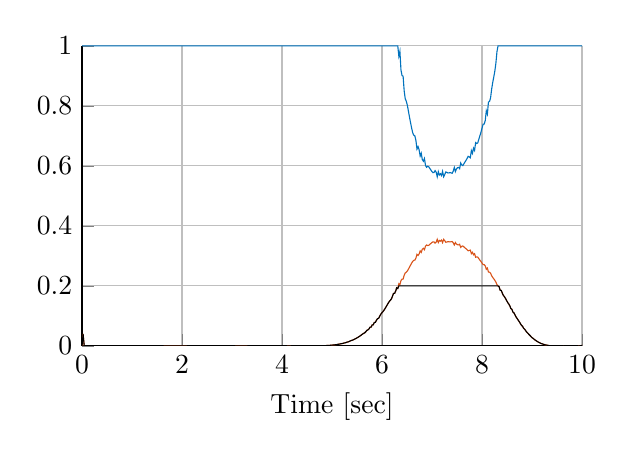
\begin{tikzpicture}

\begin{axis}[%
width=2.5in,
height=1.5in,
scale only axis,
xmin=0,
xmax=10,
xlabel={Time [sec]},
xmajorgrids,
ymin=0,
ymax=1,
ymajorgrids,
axis background/.style={fill=white},
axis x line*=bottom,
axis y line*=left
]
\addplot [color=mycolor1,solid,forget plot]
  table[row sep=crcr]{%
0	1\\
0.0213333333333333	1\\
0.0426666666666667	1\\
0.064	1\\
0.0853333333333333	1\\
0.106666666666667	1\\
0.128	1\\
0.149333333333333	1\\
0.170666666666667	1\\
0.192	1\\
0.213333333333333	1\\
0.234666666666667	1\\
0.256	1\\
0.277333333333333	1\\
0.298666666666667	1\\
0.32	1\\
0.341333333333333	1\\
0.362666666666667	1\\
0.384	1\\
0.405333333333333	1\\
0.426666666666667	1\\
0.448	1\\
0.469333333333333	1\\
0.490666666666667	1\\
0.512	1\\
0.533333333333333	1\\
0.554666666666667	1\\
0.576	1\\
0.597333333333333	1\\
0.618666666666667	1\\
0.64	1\\
0.661333333333333	1\\
0.682666666666667	1\\
0.704	1\\
0.725333333333333	1\\
0.746666666666667	1\\
0.768	1\\
0.789333333333333	1\\
0.810666666666667	1\\
0.832	1\\
0.853333333333333	1\\
0.874666666666667	1\\
0.896	1\\
0.917333333333333	1\\
0.938666666666667	1\\
0.96	1\\
0.981333333333333	1\\
1.00266666666667	1\\
1.024	1\\
1.04533333333333	1\\
1.06666666666667	1\\
1.088	1\\
1.10933333333333	1\\
1.13066666666667	1\\
1.152	1\\
1.17333333333333	1\\
1.19466666666667	1\\
1.216	1\\
1.23733333333333	1\\
1.25866666666667	1\\
1.28	1\\
1.30133333333333	1\\
1.32266666666667	1\\
1.344	1\\
1.36533333333333	1\\
1.38666666666667	1\\
1.408	1\\
1.42933333333333	1\\
1.45066666666667	1\\
1.472	1\\
1.49333333333333	1\\
1.51466666666667	1\\
1.536	1\\
1.55733333333333	1\\
1.57866666666667	1\\
1.6	1\\
1.62133333333333	1\\
1.64266666666667	1\\
1.664	1\\
1.68533333333333	1\\
1.70666666666667	1\\
1.728	1\\
1.74933333333333	1\\
1.77066666666667	1\\
1.792	1\\
1.81333333333333	1\\
1.83466666666667	1\\
1.856	1\\
1.87733333333333	1\\
1.89866666666667	1\\
1.92	1\\
1.94133333333333	1\\
1.96266666666667	1\\
1.984	1\\
2.00533333333333	1\\
2.02666666666667	1\\
2.048	1\\
2.06933333333333	1\\
2.09066666666667	1\\
2.112	1\\
2.13333333333333	1\\
2.15466666666667	1\\
2.176	1\\
2.19733333333333	1\\
2.21866666666667	1\\
2.24	1\\
2.26133333333333	1\\
2.28266666666667	1\\
2.304	1\\
2.32533333333333	1\\
2.34666666666667	1\\
2.368	1\\
2.38933333333333	1\\
2.41066666666667	1\\
2.432	1\\
2.45333333333333	1\\
2.47466666666667	1\\
2.496	1\\
2.51733333333333	1\\
2.53866666666667	1\\
2.56	1\\
2.58133333333333	1\\
2.60266666666667	1\\
2.624	1\\
2.64533333333333	1\\
2.66666666666667	1\\
2.688	1\\
2.70933333333333	1\\
2.73066666666667	1\\
2.752	1\\
2.77333333333333	1\\
2.79466666666667	1\\
2.816	1\\
2.83733333333333	1\\
2.85866666666667	1\\
2.88	1\\
2.90133333333333	1\\
2.92266666666667	1\\
2.944	1\\
2.96533333333333	1\\
2.98666666666667	1\\
3.008	1\\
3.02933333333333	1\\
3.05066666666667	1\\
3.072	1\\
3.09333333333333	1\\
3.11466666666667	1\\
3.136	1\\
3.15733333333333	1\\
3.17866666666667	1\\
3.2	1\\
3.22133333333333	1\\
3.24266666666667	1\\
3.264	1\\
3.28533333333333	1\\
3.30666666666667	1\\
3.328	1\\
3.34933333333333	1\\
3.37066666666667	1\\
3.392	1\\
3.41333333333333	1\\
3.43466666666667	1\\
3.456	1\\
3.47733333333333	1\\
3.49866666666667	1\\
3.52	1\\
3.54133333333333	1\\
3.56266666666667	1\\
3.584	1\\
3.60533333333333	1\\
3.62666666666667	1\\
3.648	1\\
3.66933333333333	1\\
3.69066666666667	1\\
3.712	1\\
3.73333333333333	1\\
3.75466666666667	1\\
3.776	1\\
3.79733333333333	1\\
3.81866666666667	1\\
3.84	1\\
3.86133333333333	1\\
3.88266666666667	1\\
3.904	1\\
3.92533333333333	1\\
3.94666666666667	1\\
3.968	1\\
3.98933333333333	1\\
4.01066666666667	1\\
4.032	1\\
4.05333333333333	1\\
4.07466666666667	1\\
4.096	1\\
4.11733333333333	1\\
4.13866666666667	1\\
4.16	1\\
4.18133333333333	1\\
4.20266666666667	1\\
4.224	1\\
4.24533333333333	1\\
4.26666666666667	1\\
4.288	1\\
4.30933333333333	1\\
4.33066666666667	1\\
4.352	1\\
4.37333333333333	1\\
4.39466666666667	1\\
4.416	1\\
4.43733333333333	1\\
4.45866666666667	1\\
4.48	1\\
4.50133333333333	1\\
4.52266666666667	1\\
4.544	1\\
4.56533333333333	1\\
4.58666666666667	1\\
4.608	1\\
4.62933333333333	1\\
4.65066666666667	1\\
4.672	1\\
4.69333333333333	1\\
4.71466666666667	1\\
4.736	1\\
4.75733333333333	1\\
4.77866666666667	1\\
4.8	1\\
4.82133333333333	1\\
4.84266666666667	1\\
4.864	1\\
4.88533333333333	1\\
4.90666666666667	1\\
4.928	1\\
4.94933333333333	1\\
4.97066666666667	1\\
4.992	1\\
5.01333333333333	1\\
5.03466666666667	1\\
5.056	1\\
5.07733333333333	1\\
5.09866666666667	1\\
5.12	1\\
5.14133333333333	1\\
5.16266666666667	1\\
5.184	1\\
5.20533333333333	1\\
5.22666666666667	1\\
5.248	1\\
5.26933333333333	1\\
5.29066666666667	1\\
5.312	1\\
5.33333333333333	1\\
5.35466666666667	1\\
5.376	1\\
5.39733333333333	1\\
5.41866666666667	1\\
5.44	1\\
5.46133333333333	1\\
5.48266666666667	1\\
5.504	1\\
5.52533333333333	1\\
5.54666666666667	1\\
5.568	1\\
5.58933333333333	1\\
5.61066666666667	1\\
5.632	1\\
5.65333333333333	1\\
5.67466666666667	1\\
5.696	1\\
5.71733333333333	1\\
5.73866666666667	1\\
5.76	1\\
5.78133333333333	1\\
5.80266666666667	1\\
5.824	1\\
5.84533333333333	1\\
5.86666666666667	1\\
5.888	1\\
5.90933333333333	1\\
5.93066666666667	1\\
5.952	1\\
5.97333333333333	1\\
5.99466666666667	1\\
6.016	1\\
6.03733333333333	1\\
6.05866666666667	1\\
6.08	1\\
6.10133333333333	1\\
6.12266666666667	1\\
6.144	1\\
6.16533333333333	1\\
6.18666666666667	1\\
6.208	1\\
6.22933333333333	1\\
6.25066666666667	1\\
6.272	1\\
6.29333333333333	1\\
6.31466666666667	1\\
6.336	0.9653280437395\\
6.35733333333333	0.981858691701559\\
6.37866666666667	0.91941644163458\\
6.4	0.900681460784169\\
6.42133333333333	0.898791515558405\\
6.44266666666667	0.849899759421221\\
6.464	0.823466828178214\\
6.48533333333333	0.814990102889263\\
6.50666666666667	0.801401737714459\\
6.528	0.781898655354693\\
6.54933333333333	0.762035673074443\\
6.57066666666667	0.743444922836831\\
6.592	0.725762623848362\\
6.61333333333333	0.710324527048778\\
6.63466666666667	0.701821482058343\\
6.656	0.700143118159379\\
6.67733333333333	0.684694463086329\\
6.69866666666667	0.655721023390825\\
6.72	0.663982857197973\\
6.74133333333333	0.653396132877242\\
6.76266666666667	0.632353643910407\\
6.784	0.641871788612843\\
6.80533333333333	0.621055652727582\\
6.82666666666667	0.615203610291529\\
6.848	0.624359838472092\\
6.86933333333333	0.601440706166282\\
6.89066666666667	0.594923707024997\\
6.912	0.598446878431474\\
6.93333333333333	0.596963942981492\\
6.95466666666667	0.591669789515793\\
6.976	0.586097786894644\\
6.99733333333333	0.580973594956362\\
7.01866666666667	0.577098577427096\\
7.04	0.577950345109223\\
7.06133333333333	0.584154459481251\\
7.08266666666667	0.578884129941937\\
7.104	0.563453253884971\\
7.12533333333333	0.580610577630614\\
7.14666666666667	0.569549593877126\\
7.168	0.573403544520537\\
7.18933333333333	0.567457516937852\\
7.21066666666667	0.581341487907051\\
7.232	0.56343720103443\\
7.25333333333333	0.570667294761365\\
7.27466666666667	0.579518998452039\\
7.296	0.578146644718076\\
7.31733333333333	0.576138728455893\\
7.33866666666667	0.576494320159001\\
7.36	0.577317306954974\\
7.38133333333333	0.576407876521265\\
7.40266666666667	0.575100271969709\\
7.424	0.582360304990858\\
7.44533333333333	0.594572566280857\\
7.46666666666667	0.580796152940491\\
7.488	0.589560669749792\\
7.50933333333333	0.593694270961209\\
7.53066666666667	0.594547705941301\\
7.552	0.590681021423024\\
7.57333333333333	0.609341883117137\\
7.59466666666667	0.602832294971325\\
7.616	0.600689297846316\\
7.63733333333333	0.606647230143905\\
7.65866666666667	0.612752964002066\\
7.68	0.618157310886169\\
7.70133333333333	0.624905642473558\\
7.72266666666667	0.631624853207863\\
7.744	0.629455107492503\\
7.76533333333333	0.62682602127786\\
7.78666666666667	0.650713536282727\\
7.808	0.641548299846129\\
7.82933333333333	0.658752103819904\\
7.85066666666667	0.651374359617088\\
7.872	0.677356883981526\\
7.89333333333333	0.674331952133753\\
7.91466666666667	0.676572822248399\\
7.936	0.688529447928394\\
7.95733333333333	0.700348429198823\\
7.97866666666667	0.711778141061645\\
8	0.725607429193488\\
8.02133333333333	0.738578414632255\\
8.04266666666667	0.739059422110585\\
8.064	0.750476389060964\\
8.08533333333333	0.783395335415332\\
8.10666666666667	0.772163480874973\\
8.128	0.812611645482887\\
8.14933333333333	0.81439741579535\\
8.17066666666667	0.826305197077286\\
8.192	0.855487270058899\\
8.21333333333333	0.877473132452843\\
8.23466666666667	0.895902013853199\\
8.256	0.915848802269921\\
8.27733333333333	0.942447186238198\\
8.29866666666667	0.980703329880243\\
8.32	1\\
8.34133333333333	1\\
8.36266666666667	1\\
8.384	1\\
8.40533333333333	1\\
8.42666666666667	1\\
8.448	1\\
8.46933333333333	1\\
8.49066666666667	1\\
8.512	1\\
8.53333333333333	1\\
8.55466666666667	1\\
8.576	1\\
8.59733333333333	1\\
8.61866666666667	1\\
8.64	1\\
8.66133333333333	1\\
8.68266666666667	1\\
8.704	1\\
8.72533333333333	1\\
8.74666666666667	1\\
8.768	1\\
8.78933333333333	1\\
8.81066666666667	1\\
8.832	1\\
8.85333333333333	1\\
8.87466666666667	1\\
8.896	1\\
8.91733333333333	1\\
8.93866666666667	1\\
8.96	1\\
8.98133333333333	1\\
9.00266666666667	1\\
9.024	1\\
9.04533333333333	1\\
9.06666666666667	1\\
9.088	1\\
9.10933333333333	1\\
9.13066666666667	1\\
9.152	1\\
9.17333333333333	1\\
9.19466666666667	1\\
9.216	1\\
9.23733333333333	1\\
9.25866666666667	1\\
9.28	1\\
9.30133333333333	1\\
9.32266666666667	1\\
9.344	1\\
9.36533333333333	1\\
9.38666666666667	1\\
9.408	1\\
9.42933333333333	1\\
9.45066666666667	1\\
9.472	1\\
9.49333333333333	1\\
9.51466666666667	1\\
9.536	1\\
9.55733333333333	1\\
9.57866666666667	1\\
9.6	1\\
9.62133333333333	1\\
9.64266666666667	1\\
9.664	1\\
9.68533333333333	1\\
9.70666666666667	1\\
9.728	1\\
9.74933333333333	1\\
9.77066666666667	1\\
9.792	1\\
9.81333333333333	1\\
9.83466666666667	1\\
9.856	1\\
9.87733333333333	1\\
9.89866666666667	1\\
9.92	1\\
9.94133333333333	1\\
9.96266666666667	1\\
9.984	1\\
10.0053333333333	1\\
};
\addplot [color=mycolor2,solid,forget plot]
  table[row sep=crcr]{%
0	0.000393103114443459\\
0.0213333333333333	0.0393915477580857\\
0.0426666666666667	0.00146511568754698\\
0.064	8.36030774515732e-05\\
0.0853333333333333	8.11176679805252e-05\\
0.106666666666667	8.278439558703e-05\\
0.128	8.73031560982029e-05\\
0.149333333333333	9.20605803312465e-05\\
0.170666666666667	9.52132286331179e-05\\
0.192	9.62244620117345e-05\\
0.213333333333333	9.55244633907065e-05\\
0.234666666666667	9.39926501886425e-05\\
0.256	9.25093024211933e-05\\
0.277333333333333	9.16603167728589e-05\\
0.298666666666667	9.16375656339722e-05\\
0.32	9.23169504411538e-05\\
0.341333333333333	9.34228560874352e-05\\
0.362666666666667	9.46749570817113e-05\\
0.384	9.58670332112705e-05\\
0.405333333333333	9.6884054299269e-05\\
0.426666666666667	9.76855374666473e-05\\
0.448	9.82790996506004e-05\\
0.469333333333333	9.86972146230631e-05\\
0.490666666666667	9.89817041102552e-05\\
0.512	9.91758761027263e-05\\
0.533333333333333	9.93222876109235e-05\\
0.554666666666667	9.94635129899748e-05\\
0.576	9.96431393637136e-05\\
0.597333333333333	9.99040722080964e-05\\
0.618666666666667	0.000100281204120521\\
0.64	0.000100786196240015\\
0.661333333333333	0.000101384545315458\\
0.682666666666667	0.000101970049850335\\
0.704	0.000102348824979068\\
0.725333333333333	0.00010225185666109\\
0.746666666666667	0.000101398058319511\\
0.768	9.96243436949984e-05\\
0.789333333333333	9.70766495181219e-05\\
0.810666666666667	9.43947491643339e-05\\
0.832	9.26991757682527e-05\\
0.853333333333333	9.3089834867379e-05\\
0.874666666666667	9.56780955894731e-05\\
0.896	9.89691423306533e-05\\
0.917333333333333	0.000100440379927536\\
0.938666666666667	9.8086026869083e-05\\
0.96	9.22120976881714e-05\\
0.981333333333333	8.65984717109152e-05\\
1.00266666666667	8.64560109970826e-05\\
1.024	9.17980008154481e-05\\
1.04533333333333	9.57626792841925e-05\\
1.06666666666667	9.22193934937868e-05\\
1.088	8.30466389792519e-05\\
1.10933333333333	7.91453831259259e-05\\
1.13066666666667	8.55666987446584e-05\\
1.152	9.00280164239099e-05\\
1.17333333333333	8.27911710533397e-05\\
1.19466666666667	7.29106351831906e-05\\
1.216	7.71110124980109e-05\\
1.23733333333333	8.37377114602232e-05\\
1.25866666666667	7.57636062042899e-05\\
1.28	6.60968486245003e-05\\
1.30133333333333	7.36562121886799e-05\\
1.32266666666667	7.53250812879496e-05\\
1.344	6.22648910667071e-05\\
1.36533333333333	6.36419998379241e-05\\
1.38666666666667	6.97478535585958e-05\\
1.408	5.75873587725975e-05\\
1.42933333333333	5.66857685467256e-05\\
1.45066666666667	6.24549196666172e-05\\
1.472	4.98667079654651e-05\\
1.49333333333333	5.21984818929534e-05\\
1.51466666666667	5.3144772788039e-05\\
1.536	4.1662761052108e-05\\
1.55733333333333	4.82762895047967e-05\\
1.57866666666667	4.00983364645556e-05\\
1.6	3.83167174391871e-05\\
1.62133333333333	3.86750928014442e-05\\
1.64266666666667	3.0084186974945e-05\\
1.664	3.37936547599372e-05\\
1.68533333333333	2.45906302401587e-05\\
1.70666666666667	2.71196084186702e-05\\
1.728	1.97664884618302e-05\\
1.74933333333333	2.02201113910977e-05\\
1.77066666666667	1.4464616262668e-05\\
1.792	1.35313812303684e-05\\
1.81333333333333	8.70745294125698e-06\\
1.83466666666667	6.89139788271158e-06\\
1.856	2.90279823866731e-06\\
1.87733333333333	1.13681741605359e-06\\
1.89866666666667	3.10922290907567e-06\\
1.92	6.93697524934423e-06\\
1.94133333333333	9.66821947588814e-06\\
1.96266666666667	1.25219524024488e-05\\
1.984	1.74922476853785e-05\\
2.00533333333333	1.75673257576689e-05\\
2.02666666666667	2.3991607514697e-05\\
2.048	2.611476102035e-05\\
2.06933333333333	2.68303178782026e-05\\
2.09066666666667	3.46013125974599e-05\\
2.112	3.49293297387465e-05\\
2.13333333333333	3.57289192087958e-05\\
2.15466666666667	4.39623915087804e-05\\
2.176	4.53285970039883e-05\\
2.19733333333333	4.37659664245671e-05\\
2.21866666666667	5.05258601156612e-05\\
2.24	5.62984654075197e-05\\
2.26133333333333	5.49302090318167e-05\\
2.28266666666667	5.46626590083086e-05\\
2.304	6.08118808707166e-05\\
2.32533333333333	6.65339497003085e-05\\
2.34666666666667	6.72063877562728e-05\\
2.368	6.56799426857858e-05\\
2.38933333333333	6.67518415466299e-05\\
2.41066666666667	7.09749958100428e-05\\
2.432	7.54105409026009e-05\\
2.45333333333333	7.795697343936e-05\\
2.47466666666667	7.86028980963055e-05\\
2.496	7.84213269180532e-05\\
2.51733333333333	7.84102300929342e-05\\
2.53866666666667	7.89542534280644e-05\\
2.56	7.99142875864059e-05\\
2.58133333333333	8.09672784879229e-05\\
2.60266666666667	8.1851979869725e-05\\
2.624	8.24399069801979e-05\\
2.64533333333333	8.27075890073782e-05\\
2.66666666666667	8.26883900996913e-05\\
2.688	8.24369704517364e-05\\
2.70933333333333	8.2007151868556e-05\\
2.73066666666667	8.14310439911323e-05\\
2.752	8.06878500201144e-05\\
2.77333333333333	7.96639317899121e-05\\
2.79466666666667	7.81332525719662e-05\\
2.816	7.58200667608686e-05\\
2.83733333333333	7.26090052214623e-05\\
2.85866666666667	6.88740586032486e-05\\
2.88	6.56205165632365e-05\\
2.90133333333333	6.38127645569288e-05\\
2.92266666666667	6.29195890001885e-05\\
2.944	6.06448391085944e-05\\
2.96533333333333	5.52717323535829e-05\\
2.98666666666667	4.86260640617562e-05\\
3.008	4.49793062442906e-05\\
3.02933333333333	4.34572444792338e-05\\
3.05066666666667	3.84625024836987e-05\\
3.072	3.06908781218238e-05\\
3.09333333333333	2.64881524898199e-05\\
3.11466666666667	2.27605627755612e-05\\
3.136	1.53538444673849e-05\\
3.15733333333333	9.77466336133498e-06\\
3.17866666666667	4.60751853120477e-06\\
3.2	3.59875350152214e-06\\
3.22133333333333	9.04595293751445e-06\\
3.24266666666667	1.69368717446728e-05\\
3.264	2.12108725709466e-05\\
3.28533333333333	3.13815855117677e-05\\
3.30666666666667	3.47829935255419e-05\\
3.328	4.54756699481723e-05\\
3.34933333333333	4.90912036542668e-05\\
3.37066666666667	6.00533850572119e-05\\
3.392	6.25797280277317e-05\\
3.41333333333333	7.5858025203948e-05\\
3.43466666666667	7.47147683202184e-05\\
3.456	9.15283459675509e-05\\
3.47733333333333	8.87249529192109e-05\\
3.49866666666667	0.000101600211000484\\
3.52	0.000109197918788123\\
3.54133333333333	0.000106535258336914\\
3.56266666666667	0.00012290254228268\\
3.584	0.00012618493999033\\
3.60533333333333	0.000123090792131973\\
3.62666666666667	0.000135687639423944\\
3.648	0.000143925087761855\\
3.66933333333333	0.00014030048245714\\
3.69066666666667	0.000140167551143864\\
3.712	0.000148041611067319\\
3.73333333333333	0.000154261552783066\\
3.75466666666667	0.000154309881294435\\
3.776	0.000151159698548003\\
3.79733333333333	0.000148523728133556\\
3.81866666666667	0.000147230849638775\\
3.84	0.000146131809319259\\
3.86133333333333	0.000144048211090626\\
3.88266666666667	0.000140492227644624\\
3.904	0.000135469095740518\\
3.92533333333333	0.000129151670749856\\
3.94666666666667	0.000121712336363077\\
3.968	0.000113272820315045\\
3.98933333333333	0.00010386416327247\\
4.01066666666667	9.3337484889011e-05\\
4.032	8.12959851441534e-05\\
4.05333333333333	6.72927913818631e-05\\
4.07466666666667	5.14971182222586e-05\\
4.096	3.53329497713026e-05\\
4.11733333333333	2.04640272633392e-05\\
4.13866666666667	8.78560588892844e-06\\
4.16	2.06965660972415e-05\\
4.18133333333333	4.11213575308711e-05\\
4.20266666666667	5.84562062196122e-05\\
4.224	8.12677184302848e-05\\
4.24533333333333	0.000108963705082318\\
4.26666666666667	0.000123815063457753\\
4.288	0.000150886127623025\\
4.30933333333333	0.000180635235008118\\
4.33066666666667	0.000189723730847528\\
4.352	0.000232265395382198\\
4.37333333333333	0.000235412636322256\\
4.39466666666667	0.000277368777331768\\
4.416	0.000278256610113459\\
4.43733333333333	0.0003206140444055\\
4.45866666666667	0.000311727885297325\\
4.48	0.000355925921127085\\
4.50133333333333	0.000344440538646883\\
4.52266666666667	0.000362683183566128\\
4.544	0.000380552287566966\\
4.56533333333333	0.000357399288632821\\
4.58666666666667	0.000362995852444891\\
4.608	0.000365668748763286\\
4.62933333333333	0.000337225511516151\\
4.65066666666667	0.00030477205040172\\
4.672	0.000277740747168064\\
4.69333333333333	0.00024204258564976\\
4.71466666666667	0.000192025476540426\\
4.736	0.000134081708234272\\
4.75733333333333	8.93270586220354e-05\\
4.77866666666667	0.000114264082306793\\
4.8	0.000204056520612996\\
4.82133333333333	0.000325073772154709\\
4.84266666666667	0.000470295434604268\\
4.864	0.000638660039003767\\
4.88533333333333	0.000828119923898503\\
4.90666666666667	0.00103354881921912\\
4.928	0.00125229195516888\\
4.94933333333333	0.00150249959441478\\
4.97066666666667	0.00182608926891166\\
4.992	0.00221292779829542\\
5.01333333333333	0.00254501037004755\\
5.03466666666667	0.00283521515024812\\
5.056	0.00338392775328367\\
5.07733333333333	0.00394293414809433\\
5.09866666666667	0.00421986011245098\\
5.12	0.00506254975854273\\
5.14133333333333	0.00552592440930282\\
5.16266666666667	0.0062308123855083\\
5.184	0.00703385871706017\\
5.20533333333333	0.00774346902129885\\
5.22666666666667	0.0085878295262161\\
5.248	0.00974622284937433\\
5.26933333333333	0.0102064771802573\\
5.29066666666667	0.0119163741421494\\
5.312	0.01278046496511\\
5.33333333333333	0.0135968813790095\\
5.35466666666667	0.0153992115388242\\
5.376	0.017023401085212\\
5.39733333333333	0.0181849527787962\\
5.41866666666667	0.0194700765950073\\
5.44	0.0211275499438221\\
5.46133333333333	0.0230102171157964\\
5.48266666666667	0.0249693766335251\\
5.504	0.0269738569555294\\
5.52533333333333	0.0290596817385545\\
5.54666666666667	0.0312949692283822\\
5.568	0.0337684123446082\\
5.58933333333333	0.0365057006407917\\
5.61066666666667	0.0392505334522518\\
5.632	0.0414582495438304\\
5.65333333333333	0.0433466874940852\\
5.67466666666667	0.0468649018682957\\
5.696	0.0515633375337839\\
5.71733333333333	0.0530568534906379\\
5.73866666666667	0.0560311040032091\\
5.76	0.0620996442974776\\
5.78133333333333	0.0621240379312981\\
5.80266666666667	0.0698128655057333\\
5.824	0.0697010434463704\\
5.84533333333333	0.0781040796411096\\
5.86666666666667	0.0780718100418584\\
5.888	0.0852157220500288\\
5.90933333333333	0.0903401841795226\\
5.93066666666667	0.0915640905500862\\
5.952	0.0979003447513516\\
5.97333333333333	0.104940200550408\\
5.99466666666667	0.109489851740075\\
6.016	0.113442828852732\\
6.03733333333333	0.11823963923855\\
6.05866666666667	0.123794345095476\\
6.08	0.129716681878509\\
6.10133333333333	0.135824654995348\\
6.12266666666667	0.141918660634248\\
6.144	0.147408703167584\\
6.16533333333333	0.151662043261489\\
6.18666666666667	0.156201009570026\\
6.208	0.165060684922731\\
6.22933333333333	0.174526482280577\\
6.25066666666667	0.174752207121522\\
6.272	0.18211619187837\\
6.29333333333333	0.193371775120194\\
6.31466666666667	0.190976111533164\\
6.336	0.20718345571443\\
6.35733333333333	0.203695299222132\\
6.37866666666667	0.217529283731789\\
6.4	0.222054087608145\\
6.42133333333333	0.222521014649035\\
6.44266666666667	0.235321869176901\\
6.464	0.242875600031719\\
6.48533333333333	0.24540175308997\\
6.50666666666667	0.24956272314855\\
6.528	0.255787624943892\\
6.54933333333333	0.262454904759376\\
6.57066666666667	0.269017910885505\\
6.592	0.275572195960572\\
6.61333333333333	0.281561444641297\\
6.63466666666667	0.284972753204174\\
6.656	0.285655882079916\\
6.67733333333333	0.29210109148317\\
6.69866666666667	0.305007759192731\\
6.72	0.301212595825148\\
6.74133333333333	0.306093026781925\\
6.76266666666667	0.316278718286846\\
6.784	0.311588705950487\\
6.80533333333333	0.322032331759047\\
6.82666666666667	0.325095621440234\\
6.848	0.320328098760215\\
6.86933333333333	0.332534858298576\\
6.89066666666667	0.336177559640596\\
6.912	0.334198417951814\\
6.93333333333333	0.33502860993767\\
6.95466666666667	0.338026384892281\\
6.976	0.341239984985563\\
6.99733333333333	0.34424972449053\\
7.01866666666667	0.346561242433951\\
7.04	0.346050489791132\\
7.06133333333333	0.342375200178403\\
7.08266666666667	0.345492283611334\\
7.104	0.354954024350759\\
7.12533333333333	0.344464961034934\\
7.14666666666667	0.351154670550337\\
7.168	0.348794495449508\\
7.18933333333333	0.352449291850519\\
7.21066666666667	0.344031871387747\\
7.232	0.354964137321452\\
7.25333333333333	0.350466903984104\\
7.27466666666667	0.345113793567118\\
7.296	0.345932994383331\\
7.31733333333333	0.347138614576422\\
7.33866666666667	0.346924493453533\\
7.36	0.346429939983764\\
7.38133333333333	0.346976521568441\\
7.40266666666667	0.347765441520316\\
7.424	0.34343000078472\\
7.44533333333333	0.336376098297019\\
7.46666666666667	0.344354897992054\\
7.488	0.33923565505969\\
7.50933333333333	0.336873724040143\\
7.53066666666667	0.336390163482938\\
7.552	0.338592222784093\\
7.57333333333333	0.328222965696834\\
7.59466666666667	0.331767228909847\\
7.616	0.332950829517141\\
7.63733333333333	0.329680892060708\\
7.65866666666667	0.326395809974941\\
7.68	0.323542238323263\\
7.70133333333333	0.320048318348258\\
7.72266666666667	0.316643651661663\\
7.744	0.317735129351353\\
7.76533333333333	0.31906780065109\\
7.78666666666667	0.307354909416088\\
7.808	0.311745818745009\\
7.82933333333333	0.303604343485601\\
7.85066666666667	0.307043095951106\\
7.872	0.295265324276906\\
7.89333333333333	0.296589831413372\\
7.91466666666667	0.29560749918295\\
7.936	0.290474141086845\\
7.95733333333333	0.285572140468415\\
7.97866666666667	0.280986431673347\\
8	0.275631136001873\\
8.02133333333333	0.270790475375024\\
8.04266666666667	0.270614234818691\\
8.064	0.266497391410609\\
8.08533333333333	0.255298941617984\\
8.10666666666667	0.259012508301184\\
8.128	0.246120026844006\\
8.14933333333333	0.245580347040613\\
8.17066666666667	0.242041319245501\\
8.192	0.233784893124395\\
8.21333333333333	0.227927206660938\\
8.23466666666667	0.223238698995459\\
8.256	0.218376657265154\\
8.27733333333333	0.212213483068802\\
8.29866666666667	0.203935271663065\\
8.32	0.199670224108211\\
8.34133333333333	0.196892078793426\\
8.36266666666667	0.185264184008457\\
8.384	0.184534304717096\\
8.40533333333333	0.175655696150527\\
8.42666666666667	0.168049254203167\\
8.448	0.163649835409242\\
8.46933333333333	0.157732502707247\\
8.49066666666667	0.151054731914214\\
8.512	0.144761269762162\\
8.53333333333333	0.139663626311036\\
8.55466666666667	0.133536238575377\\
8.576	0.12430117380577\\
8.59733333333333	0.1217517995628\\
8.61866666666667	0.112327795690382\\
8.64	0.109369225779334\\
8.66133333333333	0.102289526843853\\
8.68266666666667	0.0956912436191954\\
8.704	0.0903510341137763\\
8.72533333333333	0.0851753177532051\\
8.74666666666667	0.0798844314146447\\
8.768	0.0738262772711054\\
8.78933333333333	0.0682654154708002\\
8.81066666666667	0.0649927902936085\\
8.832	0.0582311235109634\\
8.85333333333333	0.0551857727706617\\
8.87466666666667	0.0500628883380805\\
8.896	0.045399618054053\\
8.91733333333333	0.0415454955677023\\
8.93866666666667	0.0378483585476417\\
8.96	0.0342618011852351\\
8.98133333333333	0.030487424533045\\
9.00266666666667	0.0269666799734589\\
9.024	0.0246069564788466\\
9.04533333333333	0.0210467088025604\\
9.06666666666667	0.0188858071037105\\
9.088	0.016379637382216\\
9.10933333333333	0.013998384617819\\
9.13066666666667	0.0119665914395212\\
9.152	0.0101139615880676\\
9.17333333333333	0.00838551177027982\\
9.19466666666667	0.00697205129434139\\
9.216	0.00573525946598329\\
9.23733333333333	0.00446004614196152\\
9.25866666666667	0.00352315589300075\\
9.28	0.0026795714202681\\
9.30133333333333	0.00192693592223048\\
9.32266666666667	0.00132193870919929\\
9.344	0.000834557176855952\\
9.36533333333333	0.000456170174606963\\
9.38666666666667	0.000188953160856505\\
9.408	0.000136477560500074\\
9.42933333333333	0.00025658793826862\\
9.45066666666667	0.000337138346344005\\
9.472	0.000375292443075676\\
9.49333333333333	0.00038020368122851\\
9.51466666666667	0.000354692232145468\\
9.536	0.000304152673360017\\
9.55733333333333	0.00023382271612748\\
9.57866666666667	0.000164939805114325\\
9.6	8.56034321090285e-05\\
9.62133333333333	2.43208869453194e-05\\
9.64266666666667	6.87963148049783e-05\\
9.664	0.000129379578998448\\
9.68533333333333	0.000179054884434564\\
9.70666666666667	0.000217490665650653\\
9.728	0.000249348027713889\\
9.74933333333333	0.00025449407664667\\
9.77066666666667	0.000262387437318024\\
9.792	0.000248164423972044\\
9.81333333333333	0.00022516562680456\\
9.83466666666667	0.000195260748468076\\
9.856	0.000157080100874313\\
9.87733333333333	0.000115811404105747\\
9.89866666666667	7.43877385098897e-05\\
9.92	2.95870116253147e-05\\
9.94133333333333	1.95561281518672e-05\\
9.96266666666667	5.60383677016355e-05\\
9.984	9.01502435055616e-05\\
10.0053333333333	0.00201165690933748\\
};
\addplot [color=mycolor3,solid,forget plot]
  table[row sep=crcr]{%
0	0.000393103114443459\\
0.0213333333333333	0.0393915477580857\\
0.0426666666666667	0.00146511568754698\\
0.064	8.36030774515732e-05\\
0.0853333333333333	8.11176679805252e-05\\
0.106666666666667	8.278439558703e-05\\
0.128	8.73031560982029e-05\\
0.149333333333333	9.20605803312465e-05\\
0.170666666666667	9.52132286331179e-05\\
0.192	9.62244620117345e-05\\
0.213333333333333	9.55244633907065e-05\\
0.234666666666667	9.39926501886425e-05\\
0.256	9.25093024211933e-05\\
0.277333333333333	9.16603167728589e-05\\
0.298666666666667	9.16375656339722e-05\\
0.32	9.23169504411538e-05\\
0.341333333333333	9.34228560874352e-05\\
0.362666666666667	9.46749570817113e-05\\
0.384	9.58670332112705e-05\\
0.405333333333333	9.6884054299269e-05\\
0.426666666666667	9.76855374666473e-05\\
0.448	9.82790996506004e-05\\
0.469333333333333	9.86972146230631e-05\\
0.490666666666667	9.89817041102552e-05\\
0.512	9.91758761027263e-05\\
0.533333333333333	9.93222876109235e-05\\
0.554666666666667	9.94635129899748e-05\\
0.576	9.96431393637136e-05\\
0.597333333333333	9.99040722080964e-05\\
0.618666666666667	0.000100281204120521\\
0.64	0.000100786196240015\\
0.661333333333333	0.000101384545315458\\
0.682666666666667	0.000101970049850335\\
0.704	0.000102348824979068\\
0.725333333333333	0.00010225185666109\\
0.746666666666667	0.000101398058319511\\
0.768	9.96243436949984e-05\\
0.789333333333333	9.70766495181219e-05\\
0.810666666666667	9.43947491643339e-05\\
0.832	9.26991757682527e-05\\
0.853333333333333	9.3089834867379e-05\\
0.874666666666667	9.56780955894731e-05\\
0.896	9.89691423306533e-05\\
0.917333333333333	0.000100440379927536\\
0.938666666666667	9.8086026869083e-05\\
0.96	9.22120976881714e-05\\
0.981333333333333	8.65984717109152e-05\\
1.00266666666667	8.64560109970826e-05\\
1.024	9.17980008154481e-05\\
1.04533333333333	9.57626792841925e-05\\
1.06666666666667	9.22193934937868e-05\\
1.088	8.30466389792519e-05\\
1.10933333333333	7.91453831259259e-05\\
1.13066666666667	8.55666987446584e-05\\
1.152	9.00280164239099e-05\\
1.17333333333333	8.27911710533397e-05\\
1.19466666666667	7.29106351831906e-05\\
1.216	7.71110124980109e-05\\
1.23733333333333	8.37377114602232e-05\\
1.25866666666667	7.57636062042899e-05\\
1.28	6.60968486245003e-05\\
1.30133333333333	7.36562121886799e-05\\
1.32266666666667	7.53250812879496e-05\\
1.344	6.22648910667071e-05\\
1.36533333333333	6.36419998379241e-05\\
1.38666666666667	6.97478535585958e-05\\
1.408	5.75873587725975e-05\\
1.42933333333333	5.66857685467256e-05\\
1.45066666666667	6.24549196666172e-05\\
1.472	4.98667079654651e-05\\
1.49333333333333	5.21984818929534e-05\\
1.51466666666667	5.3144772788039e-05\\
1.536	4.1662761052108e-05\\
1.55733333333333	4.82762895047967e-05\\
1.57866666666667	4.00983364645556e-05\\
1.6	3.83167174391871e-05\\
1.62133333333333	3.86750928014442e-05\\
1.64266666666667	3.0084186974945e-05\\
1.664	3.37936547599372e-05\\
1.68533333333333	2.45906302401587e-05\\
1.70666666666667	2.71196084186702e-05\\
1.728	1.97664884618302e-05\\
1.74933333333333	2.02201113910977e-05\\
1.77066666666667	1.4464616262668e-05\\
1.792	1.35313812303684e-05\\
1.81333333333333	8.70745294125698e-06\\
1.83466666666667	6.89139788271158e-06\\
1.856	2.90279823866731e-06\\
1.87733333333333	1.13681741605359e-06\\
1.89866666666667	3.10922290907567e-06\\
1.92	6.93697524934423e-06\\
1.94133333333333	9.66821947588814e-06\\
1.96266666666667	1.25219524024488e-05\\
1.984	1.74922476853785e-05\\
2.00533333333333	1.75673257576689e-05\\
2.02666666666667	2.3991607514697e-05\\
2.048	2.611476102035e-05\\
2.06933333333333	2.68303178782026e-05\\
2.09066666666667	3.46013125974599e-05\\
2.112	3.49293297387465e-05\\
2.13333333333333	3.57289192087958e-05\\
2.15466666666667	4.39623915087804e-05\\
2.176	4.53285970039883e-05\\
2.19733333333333	4.37659664245671e-05\\
2.21866666666667	5.05258601156612e-05\\
2.24	5.62984654075197e-05\\
2.26133333333333	5.49302090318167e-05\\
2.28266666666667	5.46626590083086e-05\\
2.304	6.08118808707166e-05\\
2.32533333333333	6.65339497003085e-05\\
2.34666666666667	6.72063877562728e-05\\
2.368	6.56799426857858e-05\\
2.38933333333333	6.67518415466299e-05\\
2.41066666666667	7.09749958100428e-05\\
2.432	7.54105409026009e-05\\
2.45333333333333	7.795697343936e-05\\
2.47466666666667	7.86028980963055e-05\\
2.496	7.84213269180532e-05\\
2.51733333333333	7.84102300929342e-05\\
2.53866666666667	7.89542534280644e-05\\
2.56	7.99142875864059e-05\\
2.58133333333333	8.09672784879229e-05\\
2.60266666666667	8.1851979869725e-05\\
2.624	8.24399069801979e-05\\
2.64533333333333	8.27075890073782e-05\\
2.66666666666667	8.26883900996913e-05\\
2.688	8.24369704517364e-05\\
2.70933333333333	8.2007151868556e-05\\
2.73066666666667	8.14310439911323e-05\\
2.752	8.06878500201144e-05\\
2.77333333333333	7.96639317899121e-05\\
2.79466666666667	7.81332525719662e-05\\
2.816	7.58200667608686e-05\\
2.83733333333333	7.26090052214623e-05\\
2.85866666666667	6.88740586032486e-05\\
2.88	6.56205165632365e-05\\
2.90133333333333	6.38127645569288e-05\\
2.92266666666667	6.29195890001885e-05\\
2.944	6.06448391085944e-05\\
2.96533333333333	5.52717323535829e-05\\
2.98666666666667	4.86260640617562e-05\\
3.008	4.49793062442906e-05\\
3.02933333333333	4.34572444792338e-05\\
3.05066666666667	3.84625024836987e-05\\
3.072	3.06908781218238e-05\\
3.09333333333333	2.64881524898199e-05\\
3.11466666666667	2.27605627755612e-05\\
3.136	1.53538444673849e-05\\
3.15733333333333	9.77466336133498e-06\\
3.17866666666667	4.60751853120477e-06\\
3.2	3.59875350152214e-06\\
3.22133333333333	9.04595293751445e-06\\
3.24266666666667	1.69368717446728e-05\\
3.264	2.12108725709466e-05\\
3.28533333333333	3.13815855117677e-05\\
3.30666666666667	3.47829935255419e-05\\
3.328	4.54756699481723e-05\\
3.34933333333333	4.90912036542668e-05\\
3.37066666666667	6.00533850572119e-05\\
3.392	6.25797280277317e-05\\
3.41333333333333	7.5858025203948e-05\\
3.43466666666667	7.47147683202184e-05\\
3.456	9.15283459675509e-05\\
3.47733333333333	8.87249529192109e-05\\
3.49866666666667	0.000101600211000484\\
3.52	0.000109197918788123\\
3.54133333333333	0.000106535258336914\\
3.56266666666667	0.00012290254228268\\
3.584	0.00012618493999033\\
3.60533333333333	0.000123090792131973\\
3.62666666666667	0.000135687639423944\\
3.648	0.000143925087761855\\
3.66933333333333	0.00014030048245714\\
3.69066666666667	0.000140167551143864\\
3.712	0.000148041611067319\\
3.73333333333333	0.000154261552783066\\
3.75466666666667	0.000154309881294435\\
3.776	0.000151159698548003\\
3.79733333333333	0.000148523728133556\\
3.81866666666667	0.000147230849638775\\
3.84	0.000146131809319259\\
3.86133333333333	0.000144048211090626\\
3.88266666666667	0.000140492227644624\\
3.904	0.000135469095740518\\
3.92533333333333	0.000129151670749856\\
3.94666666666667	0.000121712336363077\\
3.968	0.000113272820315045\\
3.98933333333333	0.00010386416327247\\
4.01066666666667	9.3337484889011e-05\\
4.032	8.12959851441534e-05\\
4.05333333333333	6.72927913818631e-05\\
4.07466666666667	5.14971182222586e-05\\
4.096	3.53329497713026e-05\\
4.11733333333333	2.04640272633392e-05\\
4.13866666666667	8.78560588892844e-06\\
4.16	2.06965660972415e-05\\
4.18133333333333	4.11213575308711e-05\\
4.20266666666667	5.84562062196122e-05\\
4.224	8.12677184302848e-05\\
4.24533333333333	0.000108963705082318\\
4.26666666666667	0.000123815063457753\\
4.288	0.000150886127623025\\
4.30933333333333	0.000180635235008118\\
4.33066666666667	0.000189723730847528\\
4.352	0.000232265395382198\\
4.37333333333333	0.000235412636322256\\
4.39466666666667	0.000277368777331768\\
4.416	0.000278256610113459\\
4.43733333333333	0.0003206140444055\\
4.45866666666667	0.000311727885297325\\
4.48	0.000355925921127085\\
4.50133333333333	0.000344440538646883\\
4.52266666666667	0.000362683183566128\\
4.544	0.000380552287566966\\
4.56533333333333	0.000357399288632821\\
4.58666666666667	0.000362995852444891\\
4.608	0.000365668748763286\\
4.62933333333333	0.000337225511516151\\
4.65066666666667	0.00030477205040172\\
4.672	0.000277740747168064\\
4.69333333333333	0.00024204258564976\\
4.71466666666667	0.000192025476540426\\
4.736	0.000134081708234272\\
4.75733333333333	8.93270586220354e-05\\
4.77866666666667	0.000114264082306793\\
4.8	0.000204056520612996\\
4.82133333333333	0.000325073772154709\\
4.84266666666667	0.000470295434604268\\
4.864	0.000638660039003767\\
4.88533333333333	0.000828119923898503\\
4.90666666666667	0.00103354881921912\\
4.928	0.00125229195516888\\
4.94933333333333	0.00150249959441478\\
4.97066666666667	0.00182608926891166\\
4.992	0.00221292779829542\\
5.01333333333333	0.00254501037004755\\
5.03466666666667	0.00283521515024812\\
5.056	0.00338392775328367\\
5.07733333333333	0.00394293414809433\\
5.09866666666667	0.00421986011245098\\
5.12	0.00506254975854273\\
5.14133333333333	0.00552592440930282\\
5.16266666666667	0.0062308123855083\\
5.184	0.00703385871706017\\
5.20533333333333	0.00774346902129885\\
5.22666666666667	0.0085878295262161\\
5.248	0.00974622284937433\\
5.26933333333333	0.0102064771802573\\
5.29066666666667	0.0119163741421494\\
5.312	0.01278046496511\\
5.33333333333333	0.0135968813790095\\
5.35466666666667	0.0153992115388242\\
5.376	0.017023401085212\\
5.39733333333333	0.0181849527787962\\
5.41866666666667	0.0194700765950073\\
5.44	0.0211275499438221\\
5.46133333333333	0.0230102171157964\\
5.48266666666667	0.0249693766335251\\
5.504	0.0269738569555294\\
5.52533333333333	0.0290596817385545\\
5.54666666666667	0.0312949692283822\\
5.568	0.0337684123446082\\
5.58933333333333	0.0365057006407917\\
5.61066666666667	0.0392505334522518\\
5.632	0.0414582495438304\\
5.65333333333333	0.0433466874940852\\
5.67466666666667	0.0468649018682957\\
5.696	0.0515633375337839\\
5.71733333333333	0.0530568534906379\\
5.73866666666667	0.0560311040032091\\
5.76	0.0620996442974776\\
5.78133333333333	0.0621240379312981\\
5.80266666666667	0.0698128655057333\\
5.824	0.0697010434463704\\
5.84533333333333	0.0781040796411096\\
5.86666666666667	0.0780718100418584\\
5.888	0.0852157220500288\\
5.90933333333333	0.0903401841795226\\
5.93066666666667	0.0915640905500862\\
5.952	0.0979003447513516\\
5.97333333333333	0.104940200550408\\
5.99466666666667	0.109489851740075\\
6.016	0.113442828852732\\
6.03733333333333	0.11823963923855\\
6.05866666666667	0.123794345095476\\
6.08	0.129716681878509\\
6.10133333333333	0.135824654995348\\
6.12266666666667	0.141918660634248\\
6.144	0.147408703167584\\
6.16533333333333	0.151662043261489\\
6.18666666666667	0.156201009570026\\
6.208	0.165060684922731\\
6.22933333333333	0.174526482280577\\
6.25066666666667	0.174752207121522\\
6.272	0.18211619187837\\
6.29333333333333	0.193371775120194\\
6.31466666666667	0.190976111533164\\
6.336	0.2\\
6.35733333333333	0.2\\
6.37866666666667	0.2\\
6.4	0.2\\
6.42133333333333	0.2\\
6.44266666666667	0.2\\
6.464	0.2\\
6.48533333333333	0.2\\
6.50666666666667	0.2\\
6.528	0.2\\
6.54933333333333	0.2\\
6.57066666666667	0.2\\
6.592	0.2\\
6.61333333333333	0.2\\
6.63466666666667	0.2\\
6.656	0.2\\
6.67733333333333	0.2\\
6.69866666666667	0.2\\
6.72	0.2\\
6.74133333333333	0.2\\
6.76266666666667	0.2\\
6.784	0.2\\
6.80533333333333	0.2\\
6.82666666666667	0.2\\
6.848	0.2\\
6.86933333333333	0.2\\
6.89066666666667	0.2\\
6.912	0.2\\
6.93333333333333	0.2\\
6.95466666666667	0.2\\
6.976	0.2\\
6.99733333333333	0.2\\
7.01866666666667	0.2\\
7.04	0.2\\
7.06133333333333	0.2\\
7.08266666666667	0.2\\
7.104	0.2\\
7.12533333333333	0.2\\
7.14666666666667	0.2\\
7.168	0.2\\
7.18933333333333	0.2\\
7.21066666666667	0.2\\
7.232	0.2\\
7.25333333333333	0.2\\
7.27466666666667	0.2\\
7.296	0.2\\
7.31733333333333	0.2\\
7.33866666666667	0.2\\
7.36	0.2\\
7.38133333333333	0.2\\
7.40266666666667	0.2\\
7.424	0.2\\
7.44533333333333	0.2\\
7.46666666666667	0.2\\
7.488	0.2\\
7.50933333333333	0.2\\
7.53066666666667	0.2\\
7.552	0.2\\
7.57333333333333	0.2\\
7.59466666666667	0.2\\
7.616	0.2\\
7.63733333333333	0.2\\
7.65866666666667	0.2\\
7.68	0.2\\
7.70133333333333	0.2\\
7.72266666666667	0.2\\
7.744	0.2\\
7.76533333333333	0.2\\
7.78666666666667	0.2\\
7.808	0.2\\
7.82933333333333	0.2\\
7.85066666666667	0.2\\
7.872	0.2\\
7.89333333333333	0.2\\
7.91466666666667	0.2\\
7.936	0.2\\
7.95733333333333	0.2\\
7.97866666666667	0.2\\
8	0.2\\
8.02133333333333	0.2\\
8.04266666666667	0.2\\
8.064	0.2\\
8.08533333333333	0.2\\
8.10666666666667	0.2\\
8.128	0.2\\
8.14933333333333	0.2\\
8.17066666666667	0.2\\
8.192	0.2\\
8.21333333333333	0.2\\
8.23466666666667	0.2\\
8.256	0.2\\
8.27733333333333	0.2\\
8.29866666666667	0.2\\
8.32	0.199670224108211\\
8.34133333333333	0.196892078793426\\
8.36266666666667	0.185264184008457\\
8.384	0.184534304717096\\
8.40533333333333	0.175655696150527\\
8.42666666666667	0.168049254203167\\
8.448	0.163649835409242\\
8.46933333333333	0.157732502707247\\
8.49066666666667	0.151054731914214\\
8.512	0.144761269762162\\
8.53333333333333	0.139663626311036\\
8.55466666666667	0.133536238575377\\
8.576	0.12430117380577\\
8.59733333333333	0.1217517995628\\
8.61866666666667	0.112327795690382\\
8.64	0.109369225779334\\
8.66133333333333	0.102289526843853\\
8.68266666666667	0.0956912436191954\\
8.704	0.0903510341137763\\
8.72533333333333	0.0851753177532051\\
8.74666666666667	0.0798844314146447\\
8.768	0.0738262772711054\\
8.78933333333333	0.0682654154708002\\
8.81066666666667	0.0649927902936085\\
8.832	0.0582311235109634\\
8.85333333333333	0.0551857727706617\\
8.87466666666667	0.0500628883380805\\
8.896	0.045399618054053\\
8.91733333333333	0.0415454955677023\\
8.93866666666667	0.0378483585476417\\
8.96	0.0342618011852351\\
8.98133333333333	0.030487424533045\\
9.00266666666667	0.0269666799734589\\
9.024	0.0246069564788466\\
9.04533333333333	0.0210467088025604\\
9.06666666666667	0.0188858071037105\\
9.088	0.016379637382216\\
9.10933333333333	0.013998384617819\\
9.13066666666667	0.0119665914395212\\
9.152	0.0101139615880676\\
9.17333333333333	0.00838551177027982\\
9.19466666666667	0.00697205129434139\\
9.216	0.00573525946598329\\
9.23733333333333	0.00446004614196152\\
9.25866666666667	0.00352315589300075\\
9.28	0.0026795714202681\\
9.30133333333333	0.00192693592223048\\
9.32266666666667	0.00132193870919929\\
9.344	0.000834557176855952\\
9.36533333333333	0.000456170174606963\\
9.38666666666667	0.000188953160856505\\
9.408	0.000136477560500074\\
9.42933333333333	0.00025658793826862\\
9.45066666666667	0.000337138346344005\\
9.472	0.000375292443075676\\
9.49333333333333	0.00038020368122851\\
9.51466666666667	0.000354692232145468\\
9.536	0.000304152673360017\\
9.55733333333333	0.00023382271612748\\
9.57866666666667	0.000164939805114325\\
9.6	8.56034321090285e-05\\
9.62133333333333	2.43208869453194e-05\\
9.64266666666667	6.87963148049783e-05\\
9.664	0.000129379578998448\\
9.68533333333333	0.000179054884434564\\
9.70666666666667	0.000217490665650653\\
9.728	0.000249348027713889\\
9.74933333333333	0.00025449407664667\\
9.77066666666667	0.000262387437318024\\
9.792	0.000248164423972044\\
9.81333333333333	0.00022516562680456\\
9.83466666666667	0.000195260748468076\\
9.856	0.000157080100874313\\
9.87733333333333	0.000115811404105747\\
9.89866666666667	7.43877385098897e-05\\
9.92	2.95870116253147e-05\\
9.94133333333333	1.95561281518672e-05\\
9.96266666666667	5.60383677016355e-05\\
9.984	9.01502435055616e-05\\
10.0053333333333	0.00201165690933748\\
};
\end{axis}
\end{tikzpicture}%
    \caption{Band 4 from 265 Hz to 530 Hz}
    \label{fig:Band4Simulation}
\end{subfigure}
\caption{Raw data}
\label{fig:SimulationComparisson}
\end{figure} 
